\documentclass{beamer}

% Manifest data
\input{manifest}

\usepackage{amsmath}
\usepackage{textcomp}
\usepackage{listings}
\usepackage{lmodern}
\usepackage[T1]{fontenc}
\usepackage{tikz}
\usepackage{tikzsymbols}
\usepackage{anyfontsize}

\usepackage{makecell, tabularx}
\newcolumntype{M}{>{\raggedright\arraybackslash}m}
\renewcommand\tabularxcolumn[1]{M{#1}}
\renewcommand\arraystretch{1.2}
\usetikzlibrary{shapes,shapes.geometric,arrows,graphs,graphdrawing,fit,calc,positioning,automata}
\usepackage{pgf-pie,pgfplots}
\pgfplotsset{compat=1.9}

\usepackage{multicol}

\usepackage[disable]{todonotes}
% Disable footnotes; from https://tex.stackexchange.com/a/240494/192195
\renewcommand{\footnote}[2][]{\relax}

% From https://tex.stackexchange.com/a/283202/192195
\usepackage[shortcuts]{extdash}

% Required for biblatex, but also adds functionality for quotation
\usepackage{csquotes}

% Jason's bibliography format
% % Credit to Gabriel Devenyi for this bibliography cfg:
% % github.com/gdevenyi/mcmaster.latex
% \usepackage[
%   style=numeric-comp,
%   backend=biber,
%   sorting=none,
%   backref=true,
%   maxnames=99,
%   alldates=iso,
%   seconds=true
% ]{biblatex} % bibliography
% \addbibresource{references.bib}
\usepackage[round]{natbib}
\bibliographystyle{plainnat}
\setcitestyle{yysep={;}}
\defcitealias{ISTQB}{Hamburg and Mogyorodi}
\newcommand{\citetISTQB}{\citetalias{ISTQB} (\citeyear{ISTQB})}
\newcommand{\citepISTQB}{\citepalias[\citeyear{ISTQB}]{ISTQB}}
\newcommand{\citealpISTQB}{\citetalias{ISTQB}, \citeyear{ISTQB}}

\lstset{
    language=[latex]tex,
    breaklines=true}

\usetheme{Madrid}

\setbeamertemplate{caption}{\centering\insertcaption\par}

% Change block width
\addtobeamertemplate{block begin}{%
    \centering\large%
    \setlength{\textwidth}{0.9\textwidth}
}{}

% From https://tex.stackexchange.com/a/489625/192195
\BeforeBeginEnvironment{block}{\begin{adjustbox}{minipage={\linewidth}, center}}
    \AfterEndEnvironment{block}{\end{adjustbox}}

\usepackage{adjustbox}

\def\checkmark{\tikz\fill[scale=0.4](0,.35) -- (.25,0) -- (1,.7) -- (.25,.15) -- cycle;} 

\newif\ifnotpaper

%------------------------------------------------------------------------------
% Reused in seminar slides
%------------------------------------------------------------------------------

\def\rqatext{What testing approaches do the literature describe?}
\def\rqbtext{Are these descriptions consistent?}
\def\rqctext{Can we systematically resolve any of these inconsistencies?}

\def\addTextEx{For example, \citetISTQB{} \multiAuthHelper{cite}
    \citet{GerrardAndThompson2002} as the original source
    for \ifnotpaper their \else its \fi definition of ``scalability'' (see
    \Cref{scal-test-rec}) which we verify by looking at this original source.}

\def\supers{Dr.~Spencer Smith and Dr.~Jacques Carette}
\def\supersAck{\supers{} have been great supervisors and valuable sources of
    guidance and feedback}

%------------------------------------------------------------------------------
% Spacing Options
%------------------------------------------------------------------------------

\newcommand{\thesisForceSingleSpacing}{\singlespacing}
\newcommand{\thesisForceDoubleSpacing}{\doublespacing}

%------------------------------------------------------------------------------
% Portable HREFs
%------------------------------------------------------------------------------

% Common variant
\newcommand{\porthref}[2]{\href{#2}{#1}\printOnlyFootnote{\url{#2}}}

% Custom URLs
\newcommand{\porthreft}[3]{\href{#3}{#1}\printOnlyFootnote{\href{#3}{#2}}}
% Inside of some environments, footnote marks aren't registered properly, so we
% need to manually write the "text" part
\newcommand{\porthreftm}[2]{\href{#2}{#1\printOnlyFootnoteMark}}

\newcommand{\formatPaper}[2]{%
    \ifnotpaper #1{#2}%
    \else \underline{#2}%
    \fi
}

\def\refHelper{\ifnotpaper\else Reference \fi}
\newcommand\multiAuthHelper[1]{\ifnotpaper #1\else #1s\fi}
\def\docType{\ifnotpaper thesis%
    \else paper%
    \fi}

\newcommand\flawref[1]{%
    \ifnotpaper \labelcref{#1}%
    \else \Cref{#1}%
    \fi}

\newcommand\ifblind[2]{\IfEndWith*{\jobname}{_blind}{#1}{#2}}

%------------------------------------------------------------------------------
% Generic "chunks" that get reused
%------------------------------------------------------------------------------

\def\oneSrcDistinct{we make a distinction between ``self-contained'' flaws and
    ``internal'' flaws\thesisissueref{137,138}.}

\def\highLvlScope{a high-level overview of what is in scope\ifnotpaper; see
    \Cref{app-scope} for more detailed discussion on what we include and
    exclude\fi}

\def\listAllSrcs{\ifnotpaper\ and list all sources in each tier
        in \Cref{app-src-tiers}\fi}

\newcommand\defRel[3]{We can formally define the #1 relation $#2$ on the set
    $T$ of terms used by the literature to describe test approaches based on #3.}

\NewDocumentCommand{\approachFields}{s}{%
    definitions, categories\IfBooleanTF{#1}{}{\ (see \Cref{cats-def})},
    synonyms\IfBooleanTF{#1}{}{\ (see \Cref{syn-rels})}, and
    parents\IfBooleanTF{#1}{}{\ (see \Cref{par-chd-rels})}%
}

\def\displayNL{\\
    $\,\hookrightarrow\,$\quad }

\DeclareDocumentCommand\seeSrcCode{ m m m g }{%
    (see the \href{
        https://github.com/samm82/TestingTesting/blob/#1/#2\#L#3%
        \IfNoValueF{#4}{-L#4}}
    {relevant source code})%
}

\def\ourApproachGlossary{\ifblind{our test approach glossary}{\href{
            https://github.com/samm82/TestingTesting/blob/main/ApproachGlossary.csv
        }{our test approach glossary}}}

\def\accelTolTest{astronauts \citep[p.~11]{MorgunEtAl1999}, aviators
    \citep[pp.~27, 42]{HoweAndJohnson1995}, or catalysts
    \citep[p.~1463]{LiuEtAl2023}}
\NewDocumentCommand{\orthTestIntro}{s}{%
    \IfBooleanTF{#1}{s}{S}ome test approaches appear to be combinations of
    other (seemingly orthogonal) approaches}
\def\impKeywords{``implied'', ``can be'', ``sometimes'', ``should be'',
    ``ideally'', ``usually'', ``most'', ``likely'', ``often'', ``if'', and
    ``although''\utd{}}

\def\recFigs{\Cref{fig:recoveryGraphs,fig:perf-graph}} % fig:scalGraphs

% Define common footnotes about IEEE testing terms for reuse
\newcommand{\distinctIEEE}[1]{distinct from the notion of ``test #1'' described
    in \Cref{tab:ieeeCats}.}
\newcommand{\notDefDistinctIEEE}[1]{\footnote{Not formally defined, but
        \distinctIEEE{#1}}}
% % Defined with help from GitHub Copilot
% \NewDocumentCommand{\gerrardDistinctIEEE}{s m}{%
%     \IfBooleanTF{#1}{}{\footnote}%
%     {``Each type of test addresses a different risk area''
%         \citep[p.~12]{Gerrard2000a}, which is \distinctIEEE{#2}}%
% }

\NewDocumentCommand{\multiCatIntro}{s}{%
    \IfBooleanTF{#1}{T}{we automatically detect t}est approaches with more
    than one category that violate our assumption of orthogonality
    (see \Cref{orth-approach})}

\NewDocumentCommand{\parSynFlaw}{s}{%
    \IfBooleanTF#1{P}{p}airs of synonyms where one is a subapproach of the
    other; these relations cannot coexist since synonym relations are symmetric
    while parent-child relations are asymmetric (as outlined in
    \Cref{syn-rels,par-chd-rels}, respectively).}
\NewDocumentCommand\parSynIntro{s}{%
    \IfBooleanTF#1{t}{T}here are also \parSynFlaw{}
    \IfBooleanTF#1{Below are all}{We identify} \parSynCount{}
    of these pairs\IfBooleanTF#1{\ that we identify}{} through automatic
    analysis of our generated visualizations\ifnotpaper\ as described in
        \Cref{auto-flaw-detect}\fi}

% Examples of flaws
\def\bugPattonFlaw{\citet[pp.~13\==14]{Patton2006} ``just call[s] it what it
    is and get[s] on with it'', abandoning these four terms, ``problem'',
    ``incident'', ``anomaly'', ``variance'', ``inconsistency'', ``feature'' (!),
    and ``a list of unmentionable terms'' in favour of ``bug''; after all,
    ``there's no reason to dice words''!}
\NewDocumentCommand\tourFlaw{s}{%
    \IfBooleanTF#1{t}{T}he structure of tours can be defined as either quite
    general \citep[p.~34]{IEEE2022} or ``organized around a special focus''
    \citepISTQB{}\IfBooleanTF#1{}{.}}
\def\alphaFlaw{Alpha testing is performed by ``users within the organization
    developing the software'' \citep[p.~17]{IEEE2017}, ``a small, selected
    group of potential users'' \citep[p.~5\=/8]{SWEBOK2025}, or ``roles outside
    the development organization'' conducted ``in the developer's test
    environment'' \citepISTQB{}.}
\def\loadFlaw{Load testing is performed with loads ``between anticipated
    conditions of low, typical, and peak usage'' \citep[p.~5]{IEEE2022} or
    loads that are as large as possible \citep[p.~86]{Patton2006}.}
\NewDocumentCommand{\seeRefMissing}{s}{%
    \IfBooleanTF#1{}{\refHelper} \citet[p.~42]{Kam2008} says ``See
    \emph{boundary value analysis},'' for the glossary entry of ``boundary
    value testing'' but does not include ``boundary value analysis'' in the
    glossary.}
\def\qualImprovFlaw{\citet[p.~5\=/4]{SWEBOK2025} says that quality improvement,
    along with quality assurance, is an aspect of testing that involves
    ``defining methods, tools, skills, and practices to achieve the specific
    quality level and objectives''; while testing that a system possesses
    certain qualities is in scope, actively improving the system in response is
    \emph{not} part of testing.}
\NewDocumentCommand{\tolTestFlaw}{s}{%
    \IfBooleanTF#1{t}{T}he terms ``acceleration tolerance testing'' and
    ``acoustic tolerance testing'' do not seem to refer to software testing,
    but \citet[p.~56]{Firesmith2015} includes them regardless. Elsewhere,
    they seem to refer to testing the acoustic tolerance of rats
    \citep{HolleyEtAl1996} or the acceleration tolerance of \accelTolTest{},
    which which are not relevant to software testing.}
\def\errorGuessFlaw{Since the differences between the terms ``error'',
    ``failure'', ``fault'', and ``defect'' are significant and meaningful
    \ifnotpaper (\citealp[pp.~124, 165\todo{OG 2009}, 178\==179]{IEEE2017};
        \citeyear[pp.~96, 128, 139\==140]{IEEE2010};
        \citealp[pp.~5\=/3, 12\=/3]{SWEBOK2025}\footnote{
            \citet[p.~12\=/3]{SWEBOK2025} references the definitions given in
            \citep[pp.~124, 165, 178\==179]{IEEE2017}; while we would usually
            omit the former in favour of the original source, we include it
            here as an example of a flaw within a document.};
        \citealp[pp.~399\==400]{vanVliet2000})\else TODO: make macro\fi,
    error guessing should either be called:
    \begin{itemize}
        \item ``defect guessing'' if it is based on a ``checklist of potential
              defects'' \citep[p.~29]{IEEE2021c},
        \item ``failure guessing'' if it is based on ``the tester's knowledge
              of past failures'' \citeyearpar[p.~165]{IEEE2017}, or
        \item ``fault guessing'' if it is a ``fault-based technique''
              \citep[p.~4\=/9]{SWEBOK2014} that ``anticipate[s] the most
              plausible faults in each \acs{sut}'' \citep[p.~5\=/13]{SWEBOK2025}.
    \end{itemize}
    One (or multiple) of these proposed terms may be useful in tandem with
    ``error guessing'', which would focus on errors as traditionally defined
    and be a subapproach of error-based testing (implied by
    \citealp[p.~399]{vanVliet2000}).}
\NewDocumentCommand{\perfSecParFlaw}{s}{%
    \IfBooleanTF#1{p}{P}erformance testing and security testing are given as subtypes of
    reliability testing by \citet{ISO_IEC2023a}, but these are all listed
    separately by \citet[p.~53]{Firesmith2015}.}
\def\parSheetTestFlaw{``Par sheet testing'' from \citepISTQB{} seems to refer
    to \ifnotpaper the specific example mentioned in \flawref{specific-istqb}
    \else some specific example it does not cite \fi and does not seem more
    widely applicable, since a ``PAR sheet'' is ``a list of all the symbols on
    each reel of a slot machine'' \citep{Bluejay2024}.}
\NewDocumentCommand{\redBoxFlaw}{s}{%
    \IfBooleanTF#1{t}{T}he incorrect claim that ``white-box
    testing'', ``grey-box testing'', and ``black-box testing'' are
    synonyms for ``module testing'', ``integration testing'', and
    ``system testing'', respectively, \ifnotpaper (see
        \flawref{dubious-syns}) \fi casts doubt on the claim that
    ``red-box testing'' is a synonym for ``acceptance testing''
    \citep[p.~18]{SneedAndGöschl2000}\todo{OG Hetzel88}\ifnotpaper\
        (see \flawref{dubious-red-box-syn})\fi.}

\NewDocumentCommand{\defLabelDistinct}{s}{%
    \IfBooleanTF#1{t}{T}erms can be thought of as definition-label pairs,
    but there is a meaningful distinction between definition flaws and label
    flaws}

% Used in parSyns tables
\def\ftrnote{Fault tolerance testing may also be a subapproach of
    reliability testing \ifnotpaper
        \citetext{\citealp[p.~375]{IEEE2017}; \citealp[p.~7\=/10]{SWEBOK2025}}%
    \else \cite[p.~375]{IEEE2017}, \cite[p.~7\=/10]{SWEBOK2025}%
    \fi, which is distinct from robustness testing \citep[p.~53]{Firesmith2015}.}
\def\specfn{%
    % Flaw count (MISS, SYNS): ISTQB | {IEEE2017}
    \refHelper \citetISTQB{} \multiAuthHelper{cite} \citet[p.~431]{IEEE2017}
    for \ifnotpaper their \else its \fi definition of ``functional testing''
    but \multiAuthHelper{exclude} the transitive synonym relationship
    (see \Cref{syn-rels}) \ifnotpaper they give \else it gives \fi to
    ``specification-based testing''.
    % Flaw count (CONTRA, SYNS): {IEEE2017} implied by {IEEE2021c} {IEEE2017} | {IEEE2022} {IEEE2021c} ISTQB
    % Assertion: {Kam2008} {vanVliet2000}
    These terms are also defined separately elsewhere \ifnotpaper
        (\citeyear[Fig.~2]{IEEE2022}; \citeyear[pp.~8, 49, 125]{IEEE2021c})\else
        \cite{IEEE2022}, \cite{IEEE2021c}\fi, further supporting that they are
    not synonyms.
}
\def\ucstn{%
    % Flaw count (CONTRA, SYNS): ISTQB | {IEEE2022}
    \refHelper \citet[Fig.~2]{IEEE2022} also \multiAuthHelper{list}
    ``use case testing'' and ``scenario testing'' separately, further
    supporting that these terms are not synonyms.}

%------------------------------------------------------------------------------
% For populating values from files
%------------------------------------------------------------------------------

\ExplSyntaxOn
\ior_new:N \g_hringriin_file_stream

\NewDocumentCommand{\ReadFile}{mm}
{
    \hringriin_read_file:nn { #1 } { #2 }
    \cs_new:Npn #1 ##1
    {
        \str_if_eq:nnTF { ##1 } { * }
        { \seq_count:c { g_hringriin_file_ \cs_to_str:N #1 _seq } }
        { \seq_item:cn { g_hringriin_file_ \cs_to_str:N #1 _seq } { ##1 } }
    }
}

\cs_new_protected:Nn \hringriin_read_file:nn
{
    \ior_open:Nn \g_hringriin_file_stream { #2 }
    \seq_gclear_new:c { g_hringriin_file_ \cs_to_str:N #1 _seq }
    \ior_map_inline:Nn \g_hringriin_file_stream
    {
        \seq_gput_right:cx
        { g_hringriin_file_ \cs_to_str:N #1 _seq }
        { \tl_trim_spaces:n { ##1 } }
    }
    \ior_close:N \g_hringriin_file_stream
}

\ExplSyntaxOff

% Define/read values for Undefined Terms methodology for reuse and calculation!
\ReadFile{\undefTermCounts}{assets/misc/undefTermCounts}

\newcount\TotalBefore
\newcount\UndefBefore
\newcount\TotalAfter
\newcount\UndefAfter

\TotalBefore=\undefTermCounts{1}
\UndefBefore=\undefTermCounts{2}
\TotalAfter=\undefTermCounts{3}
\UndefAfter=\undefTermCounts{4}

\def\approachCount{\undefTermCounts{3}}

\ReadFile{\qualityCounts}{build/qualityCount}
\def\qualityCount{\qualityCounts{1}}

\ReadFile{\multiCatCounts}{build/multiCatCounts}
\def\multiCatCount{\multiCatCounts{1}}
\def\multiCatMax{\multiCatCounts{2}}
\def\multiCatMaxCount{\multiCatCounts{3}}

\ReadFile{\multiSynCounts}{build/multiSynCounts}
\def\multiSynCount{\multiSynCounts{1}}

\ReadFile{\parSynCounts}{build/parSynCounts}
\def\parSynCount{\parSynCounts{1}}
\def\selfParCount{\parSynCounts{2}}

\ReadFile{\stdSources}{build/stdSources}
\ReadFile{\metaSources}{build/metaSources}
\ReadFile{\textSources}{build/textSources}
\ReadFile{\paperSources}{build/paperSources}

\def\srcCount{\the\numexpr\stdSources{3} + \metaSources{3} + \textSources{3} + \paperSources{3}}
\def\undefPerc{\the\numexpr 100 * \UndefAfter / \TotalAfter}

\ReadFile{\stdFlawDmnBrkdwn}{build/stdFlawDmnBrkdwn}
\ReadFile{\metaFlawDmnBrkdwn}{build/metaFlawDmnBrkdwn}
\ReadFile{\textFlawDmnBrkdwn}{build/textFlawDmnBrkdwn}
\ReadFile{\paperFlawDmnBrkdwn}{build/paperFlawDmnBrkdwn}
\ReadFile{\totalFlawDmnBrkdwn}{build/totalFlawDmnBrkdwn}

\ReadFile{\stdFlawMnfstBrkdwn}{build/stdFlawMnfstBrkdwn}
\ReadFile{\metaFlawMnfstBrkdwn}{build/metaFlawMnfstBrkdwn}
\ReadFile{\textFlawMnfstBrkdwn}{build/textFlawMnfstBrkdwn}
\ReadFile{\paperFlawMnfstBrkdwn}{build/paperFlawMnfstBrkdwn}
\ReadFile{\totalFlawMnfstBrkdwn}{build/totalFlawMnfstBrkdwn}

\def\flawCount{\totalFlawMnfstBrkdwn{13}}

\def\stds{\nameref{stds}}
\def\metas{\nameref{metas}}
\def\texts{\nameref{texts}}
\NewDocumentCommand{\papers}{s}{%
    \IfBooleanTF{#1}{\hyperref[papers]{Papers and Others}}{\nameref{papers}}%
}

\def\srcTier{\hyperref[source-tiers]{Source Tier}}

\input{build/FlawDmnMacros}
\input{build/FlawMnfstMacros}

% Assisted by GitHub Copilot
\newcommand\macro[2][]{\texttt{\textbackslash#2\{#1\}}}

%------------------------------------------------------------------------------
% TODOs
%------------------------------------------------------------------------------

% Generic Inlined TODOs
\newcommand{\intodo}[1]{\todo[inline]{#1}}

% Unimportant TODOs for "later" (i.e., finishing touches or changes immediately before submission)
\newcommand{\latertodo}[1]{\todo[backgroundcolor=Cyan]{\textit{Later}: #1}}

% "Important" TODOs
\newcommand{\imptodo}[1]{\todo[inline,backgroundcolor=Red]{\textbf{Important}: #1}}

% "Easy" TODOs
\newcommand{\easytodo}[1]{\todo[inline,backgroundcolor=SeaGreen]{\textit{Easy}: #1}}
\newcommand{\eztodo}[1]{\easytodo{#1}}

% "Tedious" TODOs
\newcommand{\tedioustodo}[1]{\todo[inline,backgroundcolor=PineGreen]{\textit{Needs time}: #1}}

% "Question" TODO Notes
\newcounter{todonoteQuestionsCtr}
\newcommand{\questiontodo}[1]{\stepcounter{todonoteQuestionsCtr}\todo[backgroundcolor=Lavender]{\textbf{Q \#\thetodonoteQuestionsCtr{}}: #1}}
\newcommand{\qtodo}[1]{\questiontodo{#1}}

% Specific categories of TODOs
\def\utd{\latertodo{Ensure this is up to date}}

%------------------------------------------------------------------------------
% Link to Drasil issue
%------------------------------------------------------------------------------

\newcommand{\issueref}[1]{\href{https://github.com/JacquesCarette/Drasil/issues/#1}{\##1}}
\newcommand{\pullref}[1]{\href{https://github.com/JacquesCarette/Drasil/pull/#1}{\##1}}
\newcommand{\thesisissuerefhelper}[1]{\href{https://github.com/samm82/TestingTesting/issues/#1}{\##1}}

\ExplSyntaxOn

% Based on output from ChatGPT
\NewDocumentCommand{\mapthesisissueref}{m}
{
    % Clear temporary sequences to store transformed items
    \seq_clear:N \l_tmpa_seq
    \seq_clear:N \l_tmpb_seq

    \seq_set_split:Nnn \l_tmpa_seq { , } { #1 } % Split the input by commas
    \seq_map_inline:Nn \l_tmpa_seq
    {
        \seq_put_right:Nn \l_tmpb_seq {\thesisissuerefhelper{##1}}
    }
    \seq_use:Nnnn \l_tmpb_seq { ~and~ } { ,~ } { ,~and~ }
}

\ExplSyntaxOff

\newcommand{\thesisissueref}[1]{\todo[backgroundcolor=lightgray]{See \mapthesisissueref{#1}}}

%------------------------------------------------------------------------------
% Code
%------------------------------------------------------------------------------

\input{assets/code/names}
\input{assets/misc/posterHelpers}

% for assets/code/example.tex...
\newcommand{\exampleCode}{\input{assets/code/example}}
\newcommand{\refExampleCode}{\Cref{lst:exampleCode}}

% for assets/code/examplePseudocode.tex...
\newcommand{\examplePseudocode}{\input{assets/code/examplePseudocode}}
\newcommand{\refExamplePseudocode}{\Cref{lst:examplePseudocode}}

% for assets/code/mainInvalidInputTest.tex...
\newcommand{\mainInvalidInputTest}{\input{assets/code/mainInvalidInputTest}}
\newcommand{\refMainInvalidInputTest}{\Cref{lst:mainInvalidInputTest}}

% for assets/code/projManualViolationReq.tex...
\newcommand{\projManualViolationReq}{\input{assets/code/projManualViolationReq}}
\newcommand{\refProjManualViolationReq}{\Cref{lst:projManualViolationReq}}

% for assets/code/projViolationChoice.tex...
\newcommand{\projViolationChoice}{\input{assets/code/projViolationChoice}}
\newcommand{\refProjViolationChoice}{\Cref{lst:projViolationChoice}}

%------------------------------------------------------------------------------
% Graphs
%------------------------------------------------------------------------------

% Organization of files

\newcommand{\parChdGraphs}{
    % Only top or bottom to comply with IEEE guidelines
    \begin{figure}[b!]
        \centering
        \begin{subfigure}[b]{\linewidth}
            \centering
            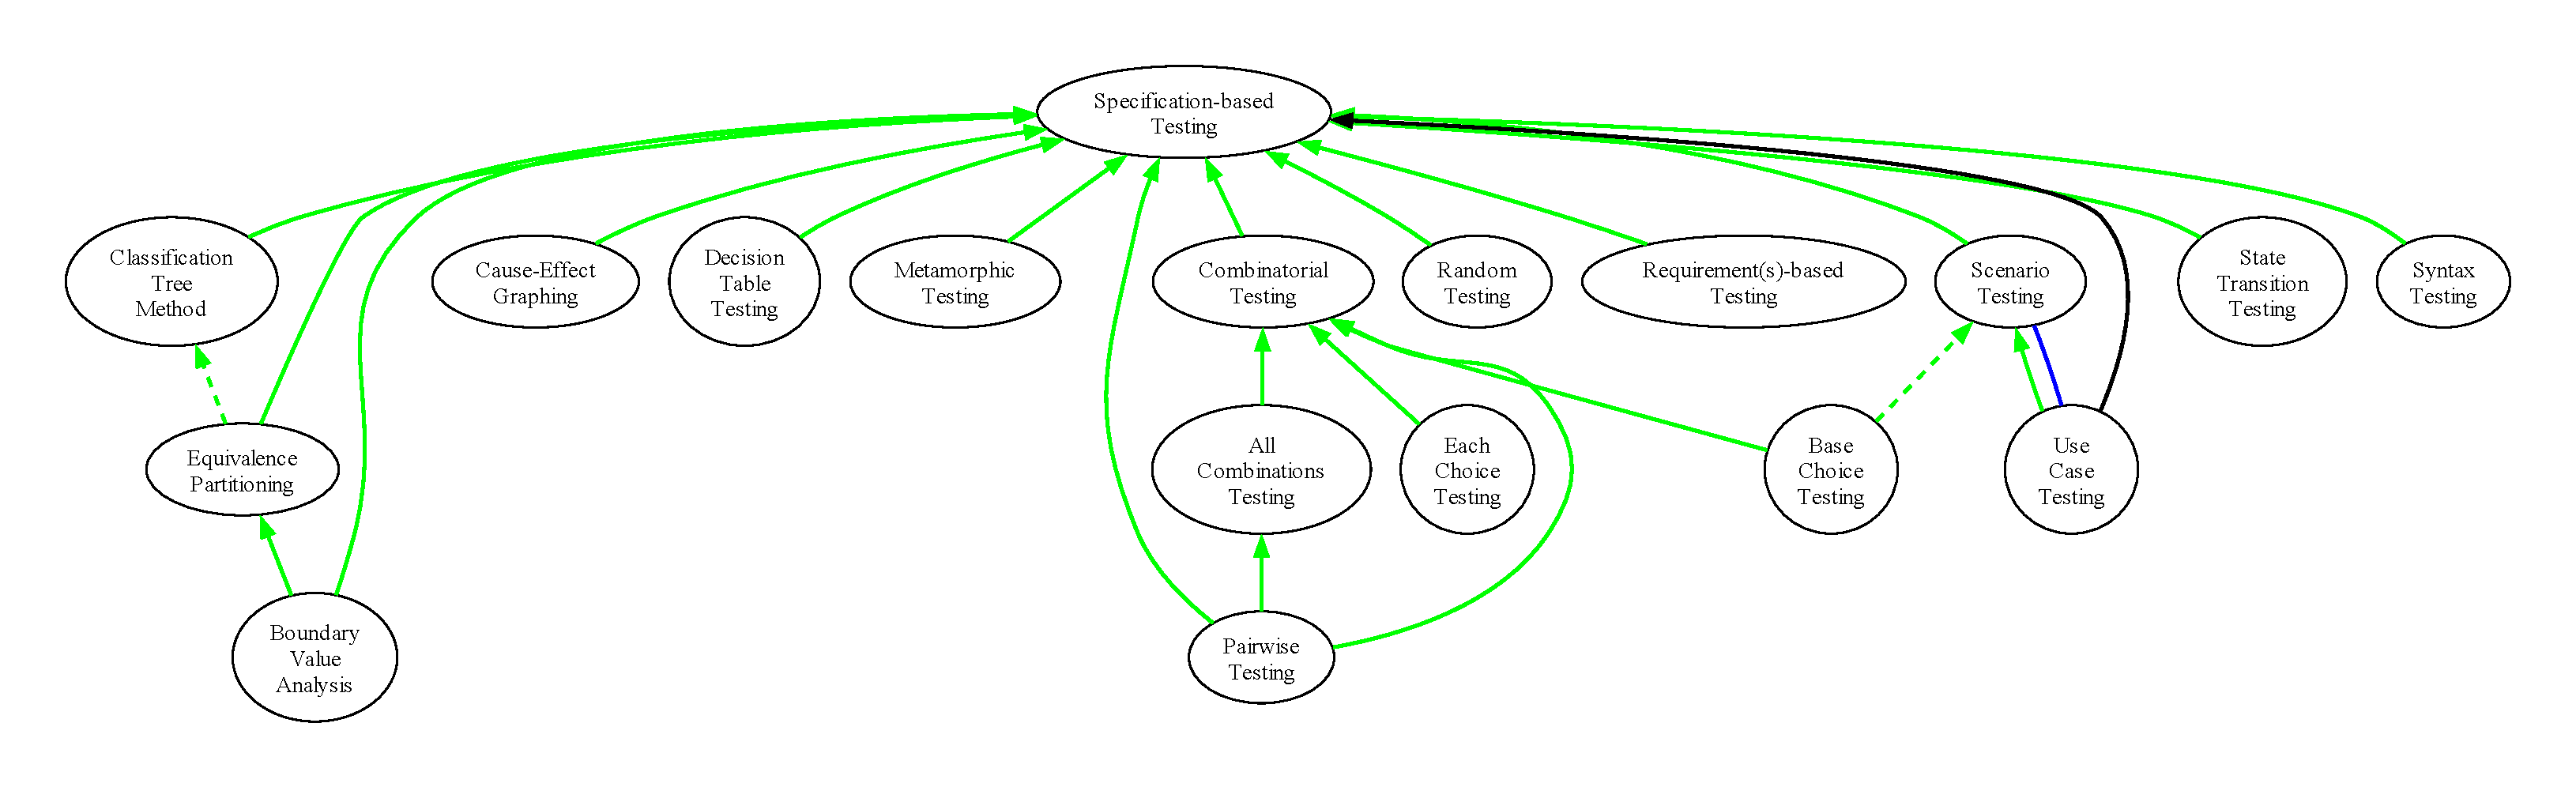
\includegraphics[width=\linewidth]{assets/graphs/specBasedGraph.pdf}
            \caption{``Superset'' relations.}
            \label{fig:specBasedGraph}
        \end{subfigure}
        \begin{subfigure}[t]{.45\linewidth}
            \centering
            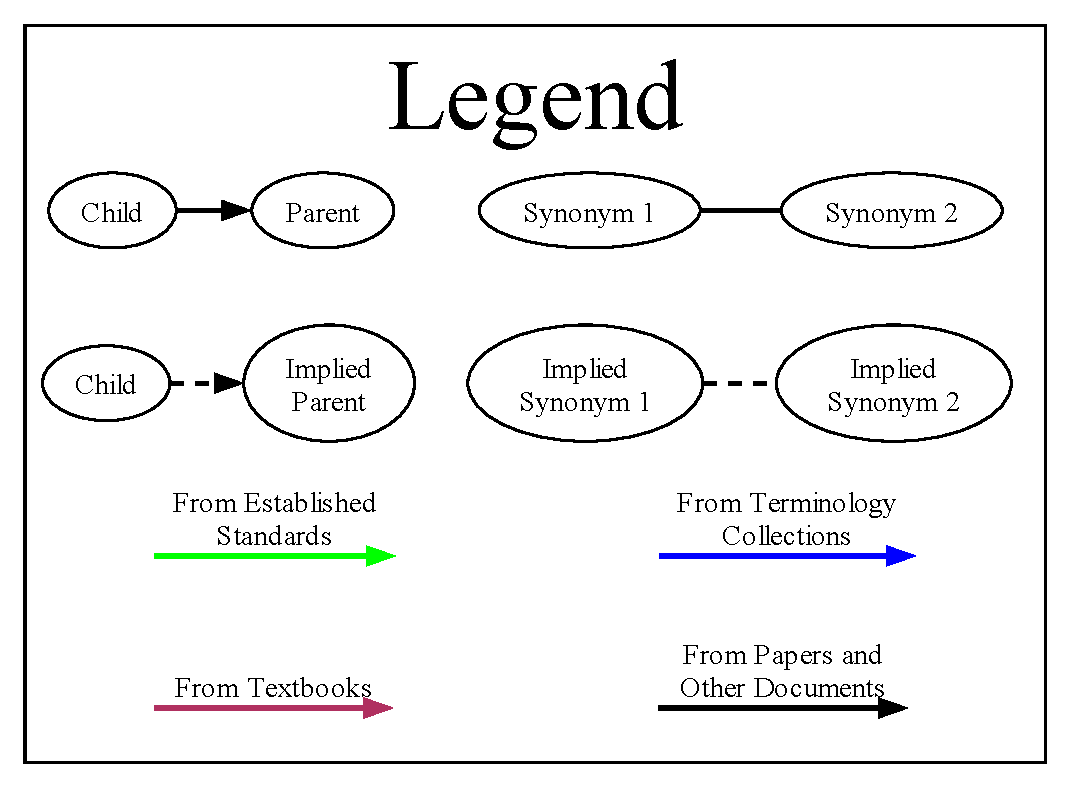
\includegraphics[width=\linewidth]{assets/graphs/parChdLegend.pdf}
        \end{subfigure}
        \begin{subfigure}[t]{.5\linewidth}
            \centering
            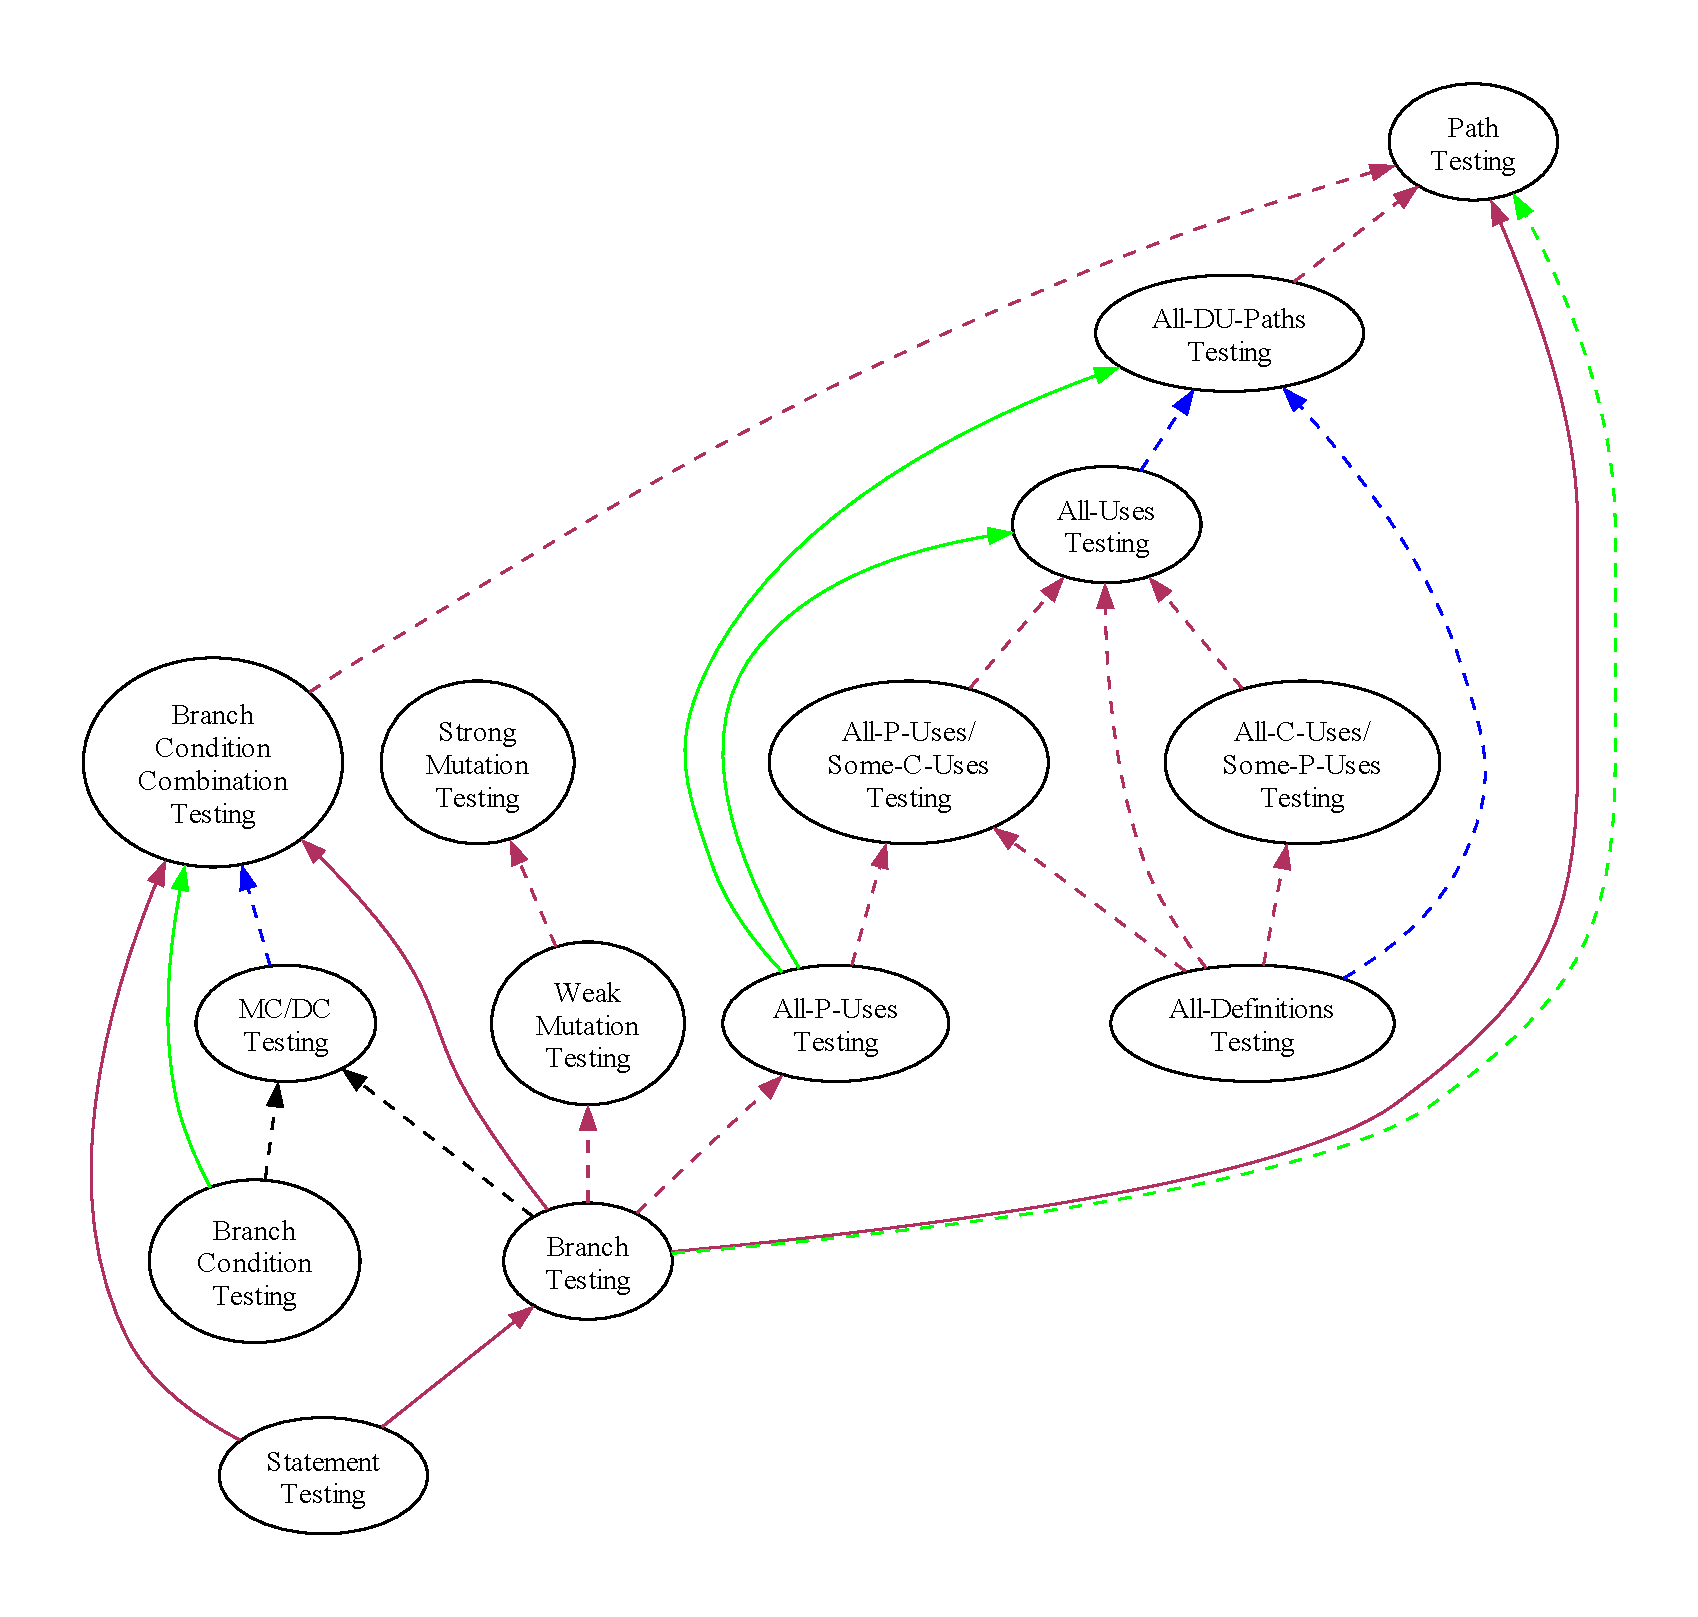
\includegraphics[width=\linewidth]{assets/graphs/subsumesGraph.pdf}
            \caption{``Subsume'' relations.}
            \label{fig:subsumesGraph}
        \end{subfigure}
        \caption{Graphs of different classes of parent-child relations.}
        \label{fig:parChdGraphs}
    \end{figure}
}

\newcommand{\ExampleGraph}{
    \begin{figure*}
        \begin{subfigure}[b]{0.275\linewidth}
            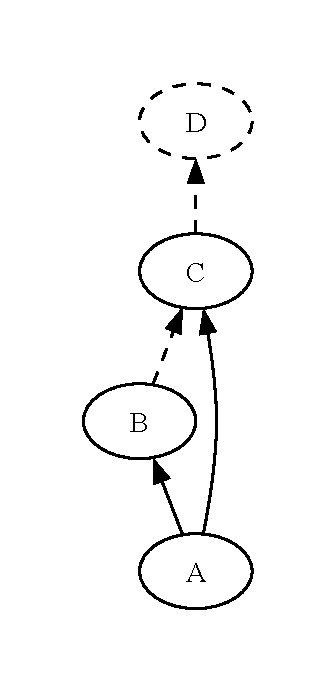
\includegraphics[width=\linewidth]{assets/graphs/ExampleGlossaryGraph.pdf}
            \caption{Graph from \\ \Cref{tab:exampleGlossary}.}
            \label{fig:exampleGraph}
        \end{subfigure}
        \centering
        \begin{subfigure}[b]{0.7\linewidth}
            \centering
            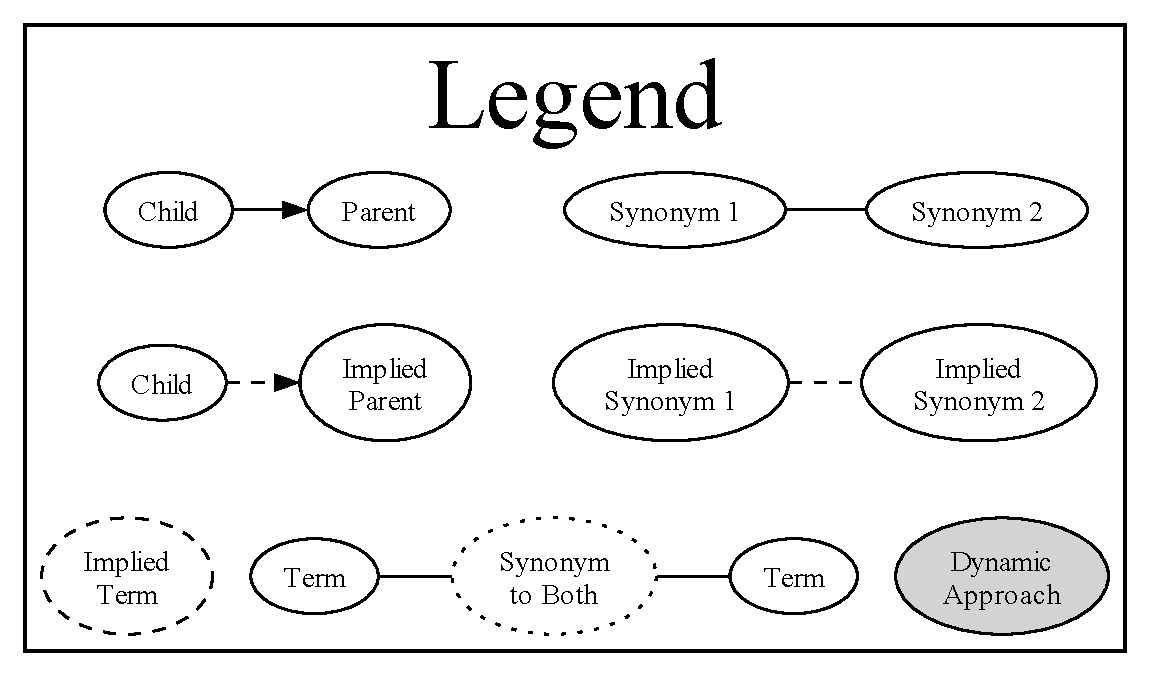
\includegraphics[width=\linewidth]{assets/graphs/manual/manualLegend.pdf}
            \hspace{5cm}\begin{subfigure}[t]{0.475\linewidth}
                \includegraphics[width=1.1\linewidth]{assets/graphs/rigidExampleGlossaryGraph.pdf}
                \caption{Rigid graph from\\\Cref{tab:exampleGlossary}.}
                \label{fig:rigidExampleGraph}
            \end{subfigure}
            \begin{subfigure}[t]{0.475\linewidth}
                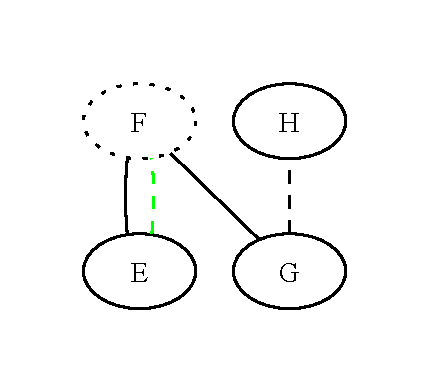
\includegraphics[width=1.1\linewidth]{assets/graphs/SynExampleGlossaryGraph.pdf}
                \caption{Graph from \Cref{tab:synExampleGlossary}.}
                \label{fig:synExampleGraph}
            \end{subfigure}
        \end{subfigure}
        \begin{subfigure}[t]{0.25\linewidth}
            \centering
            \includegraphics[width=1.2\linewidth]{assets/graphs/SelfExampleGlossaryGraph.pdf}
            \caption{Self-loop graph.}
            \label{fig:selfExampleGraph}
        \end{subfigure}
        \hfill
        \begin{subfigure}[t]{0.425\linewidth}
            \centering
            \includegraphics[width=0.6\linewidth]{assets/graphs/ParSynExampleGlossaryGraph.pdf}
            \caption{Graph of a pair of terms with a \hyperref[par-chd-rels]{parent-child} \emph{and} synonym relation.}
            \label{fig:parSynExampleGraph}
        \end{subfigure}
        \hfill
        \begin{subfigure}[t]{0.25\linewidth}
            \centering
            \includegraphics[width=1.4\linewidth]{assets/graphs/StaticExampleGlossaryGraph.pdf}
            \caption{Static graph.}
            \label{fig:staticExampleGraph}
        \end{subfigure}
        \caption{Example generated graphs.}
        \label{fig:exampleGraphs}
    \end{figure*}
}

\newcommand{\recoveryGraphs}{
    % Only top or bottom to comply with IEEE guidelines
    \begin{figure}[bt!]
        \centering
        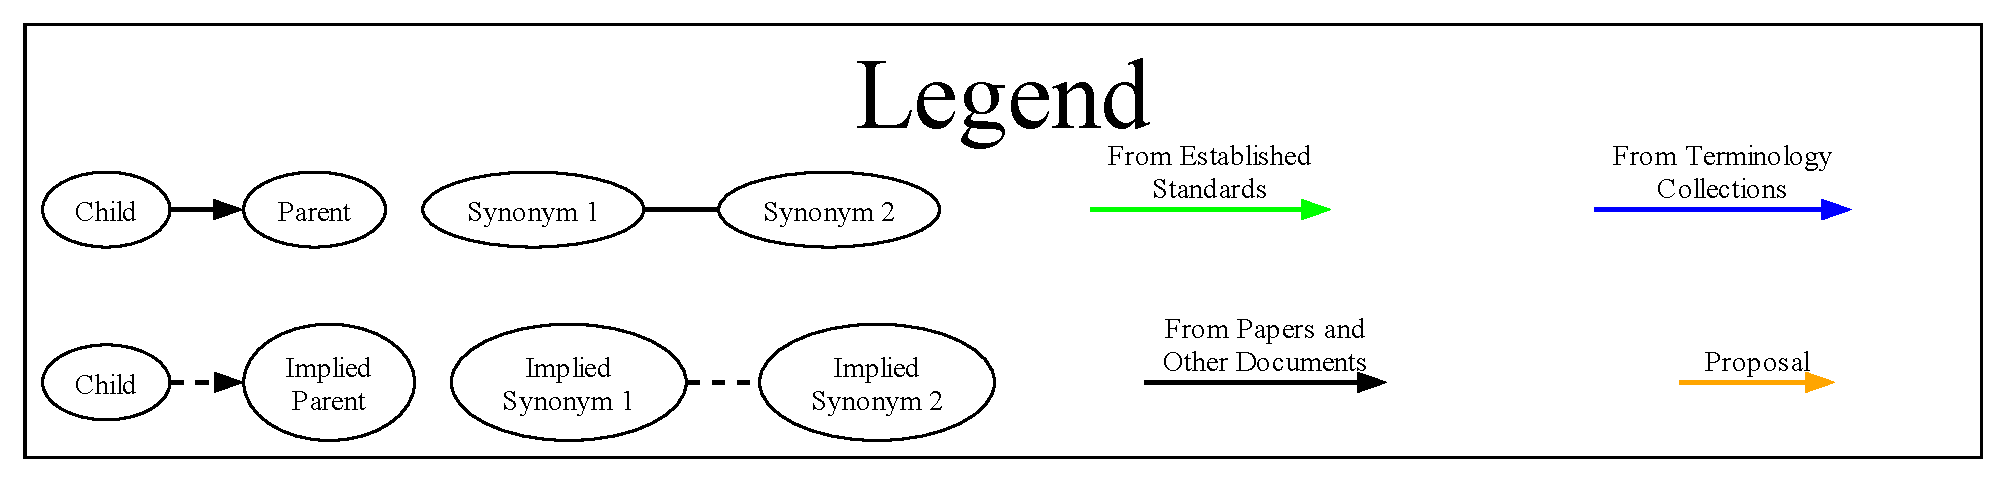
\includegraphics[width=\linewidth]{assets/graphs/recoveryLegend.pdf}
        \begin{subfigure}[b]{.475\linewidth}
            \centering
            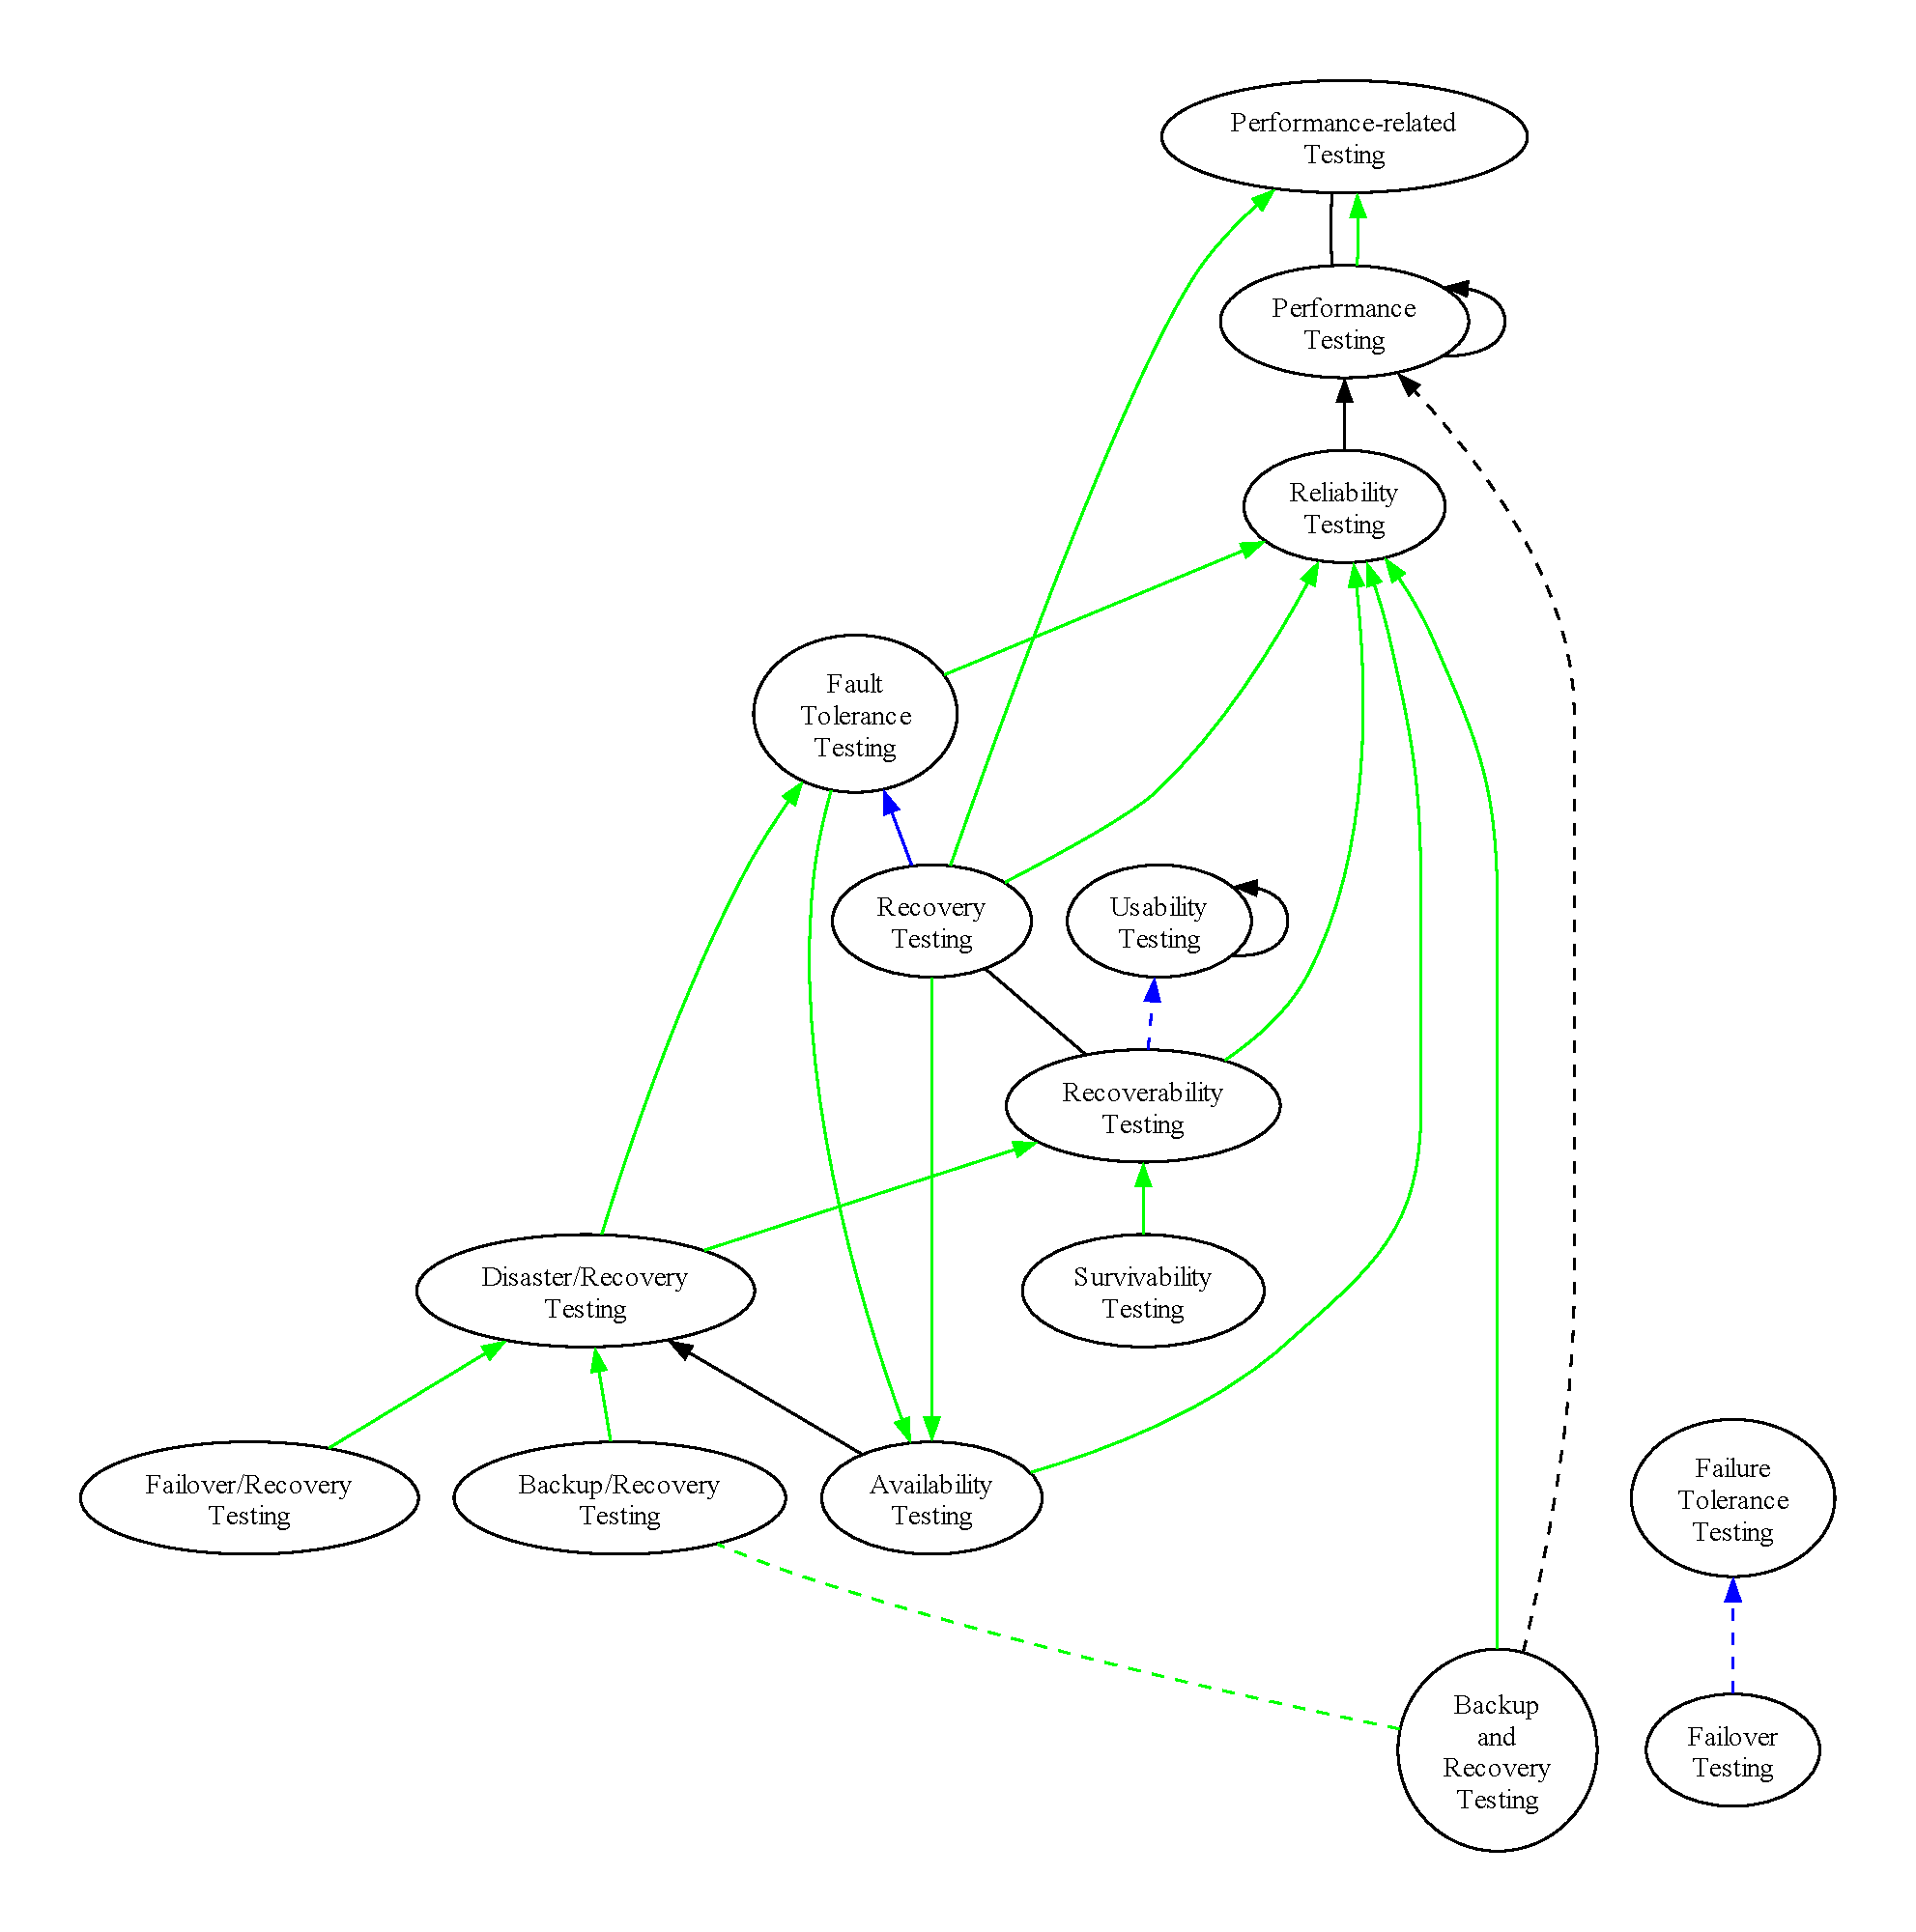
\includegraphics[width=\linewidth]{assets/graphs/recoveryGraph.pdf}
            \caption{Graph of current relations.}
            \label{fig:rec-graph-current}
        \end{subfigure}
        \begin{subfigure}[b]{.475\linewidth}
            \centering
            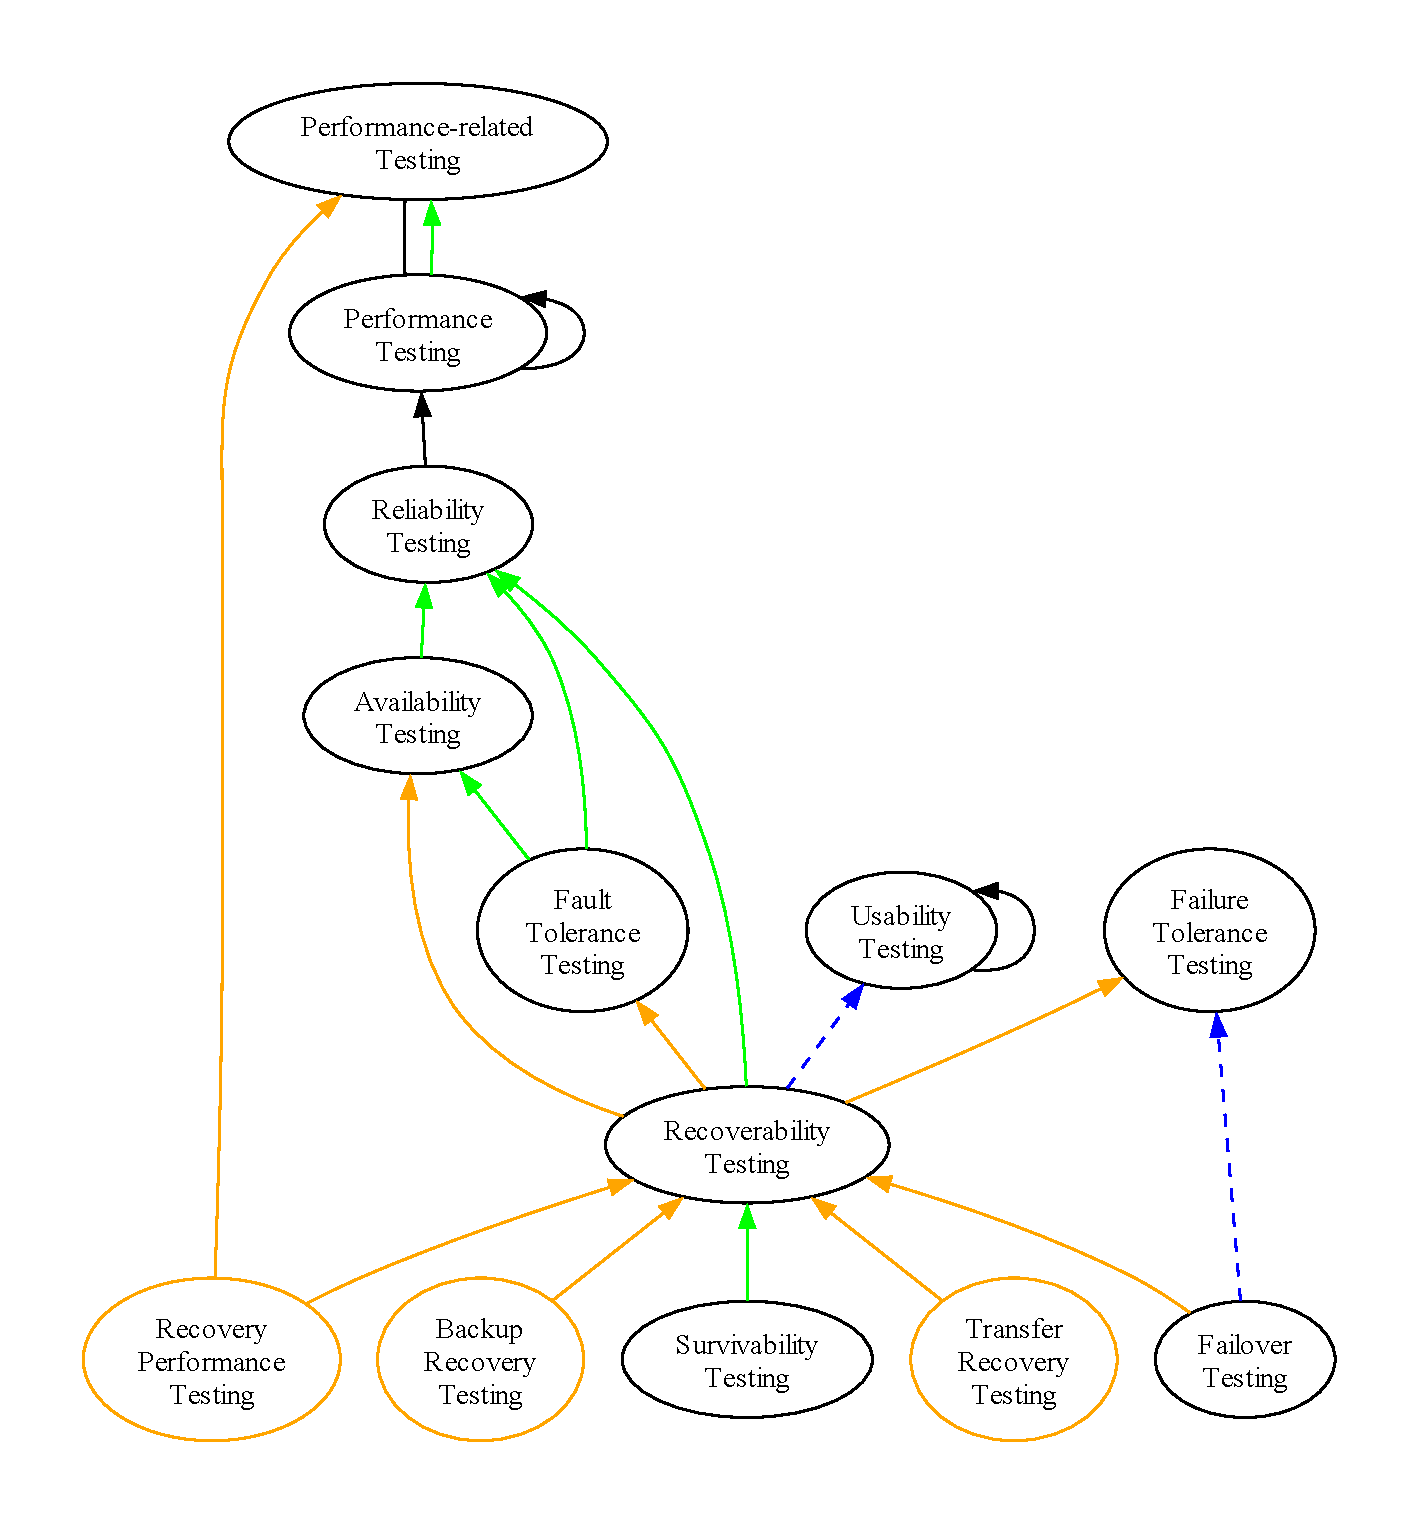
\includegraphics[width=\linewidth]{assets/graphs/recoveryProposedGraph.pdf}
            \caption{Graph of proposed relations.}
            \label{fig:rec-graph-proposed}
        \end{subfigure}
        \caption{Graphs of relations between terms related to recovery testing.}
        \label{fig:recoveryGraphs}
    \end{figure}
}

\newcommand{\scalGraphs}{
    % Only top or bottom to comply with IEEE guidelines
    \begin{figure}[b!]
        \centering
        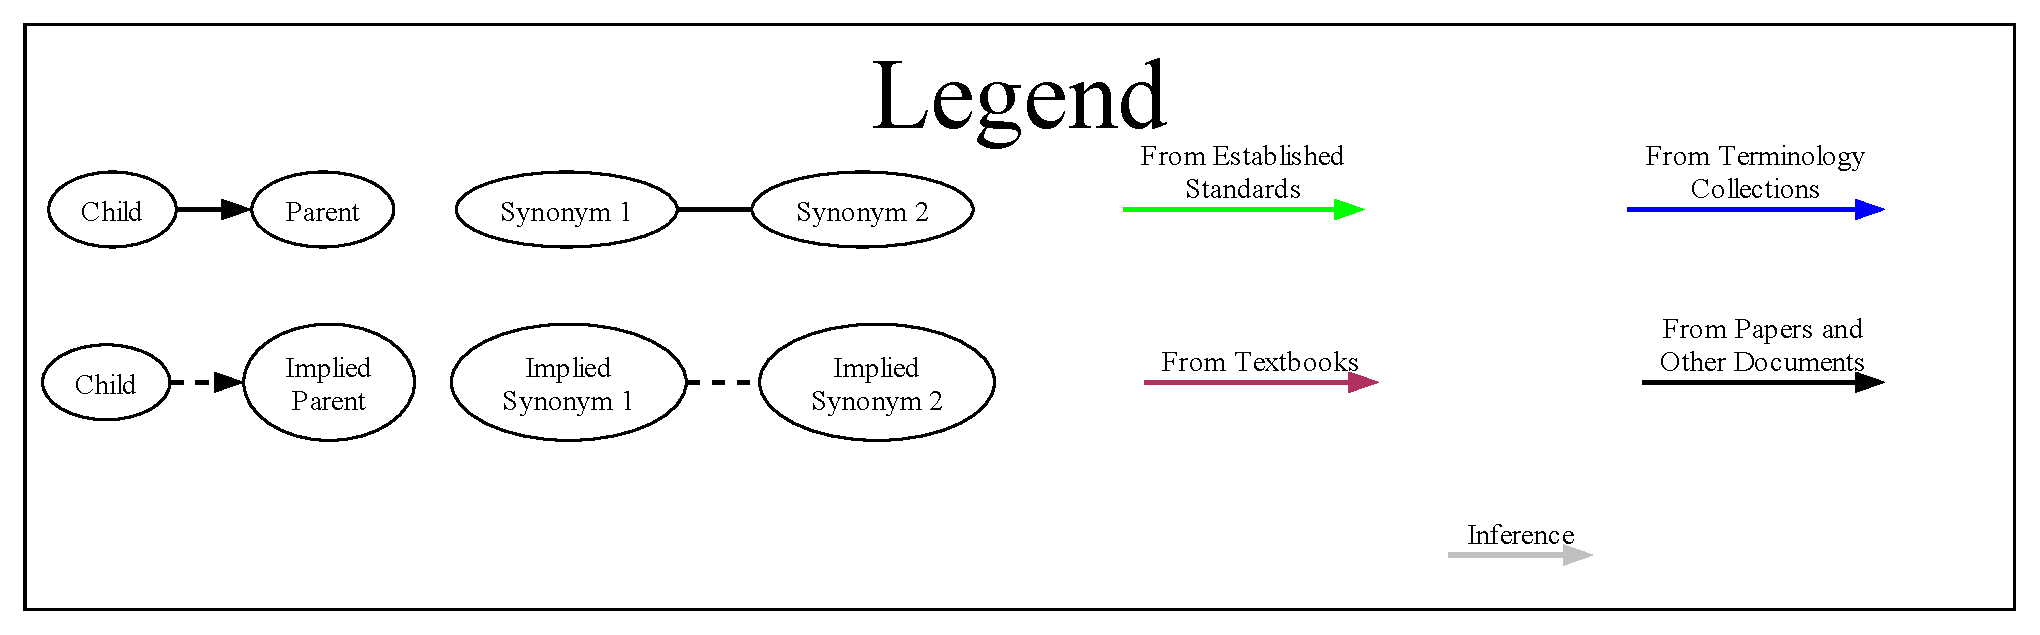
\includegraphics[width=\linewidth]{assets/graphs/scalabilityLegend.pdf}
        \begin{subfigure}[b]{.475\linewidth}
            \centering
            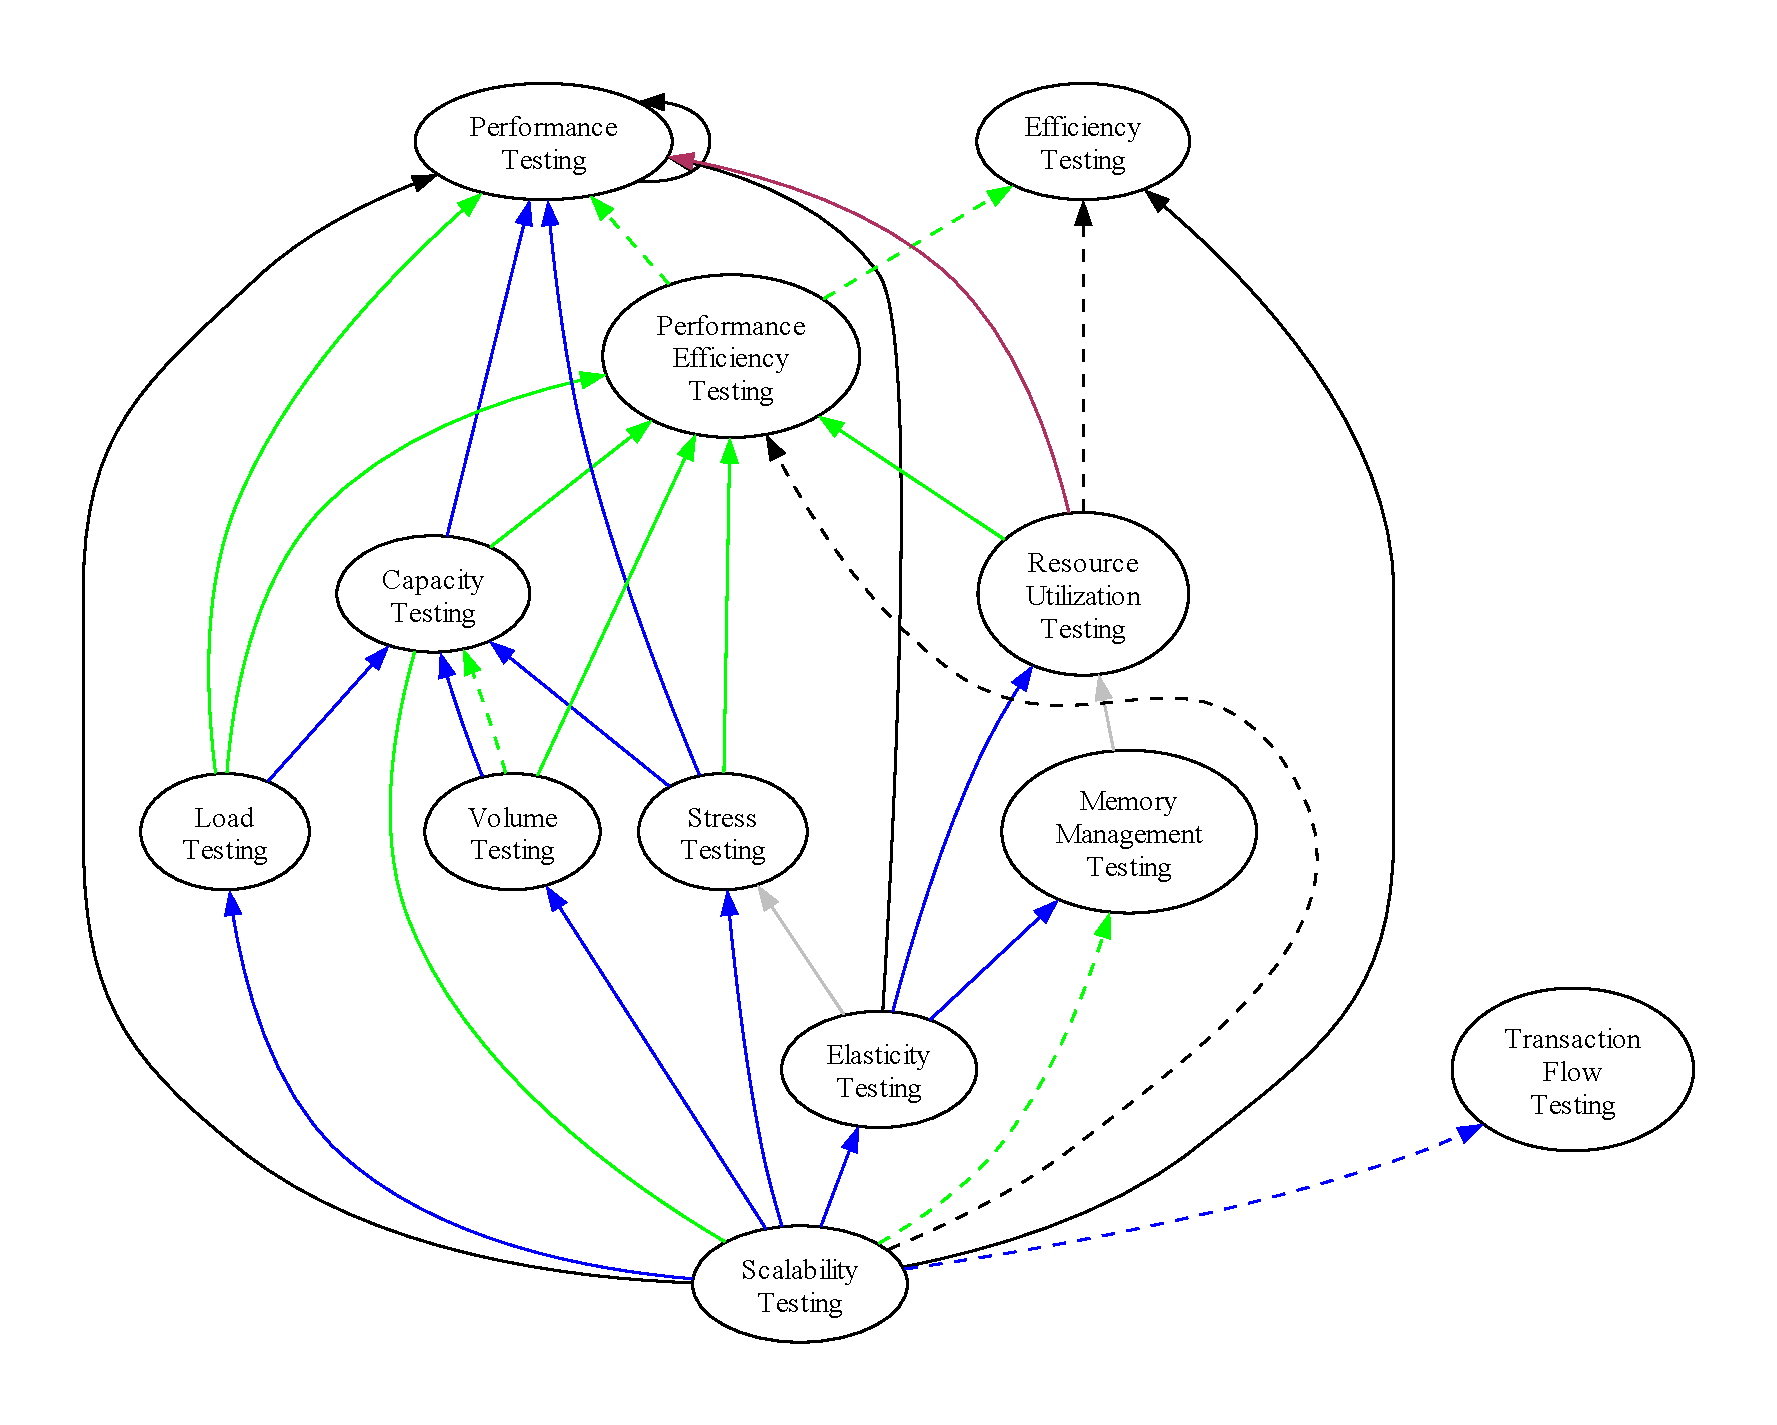
\includegraphics[width=\linewidth]{assets/graphs/scalabilityGraph.pdf}
            \caption{Graph of current relations.}
            \label{fig:scal-graph-current}
        \end{subfigure}
        \begin{subfigure}[b]{.475\linewidth}
            \centering
            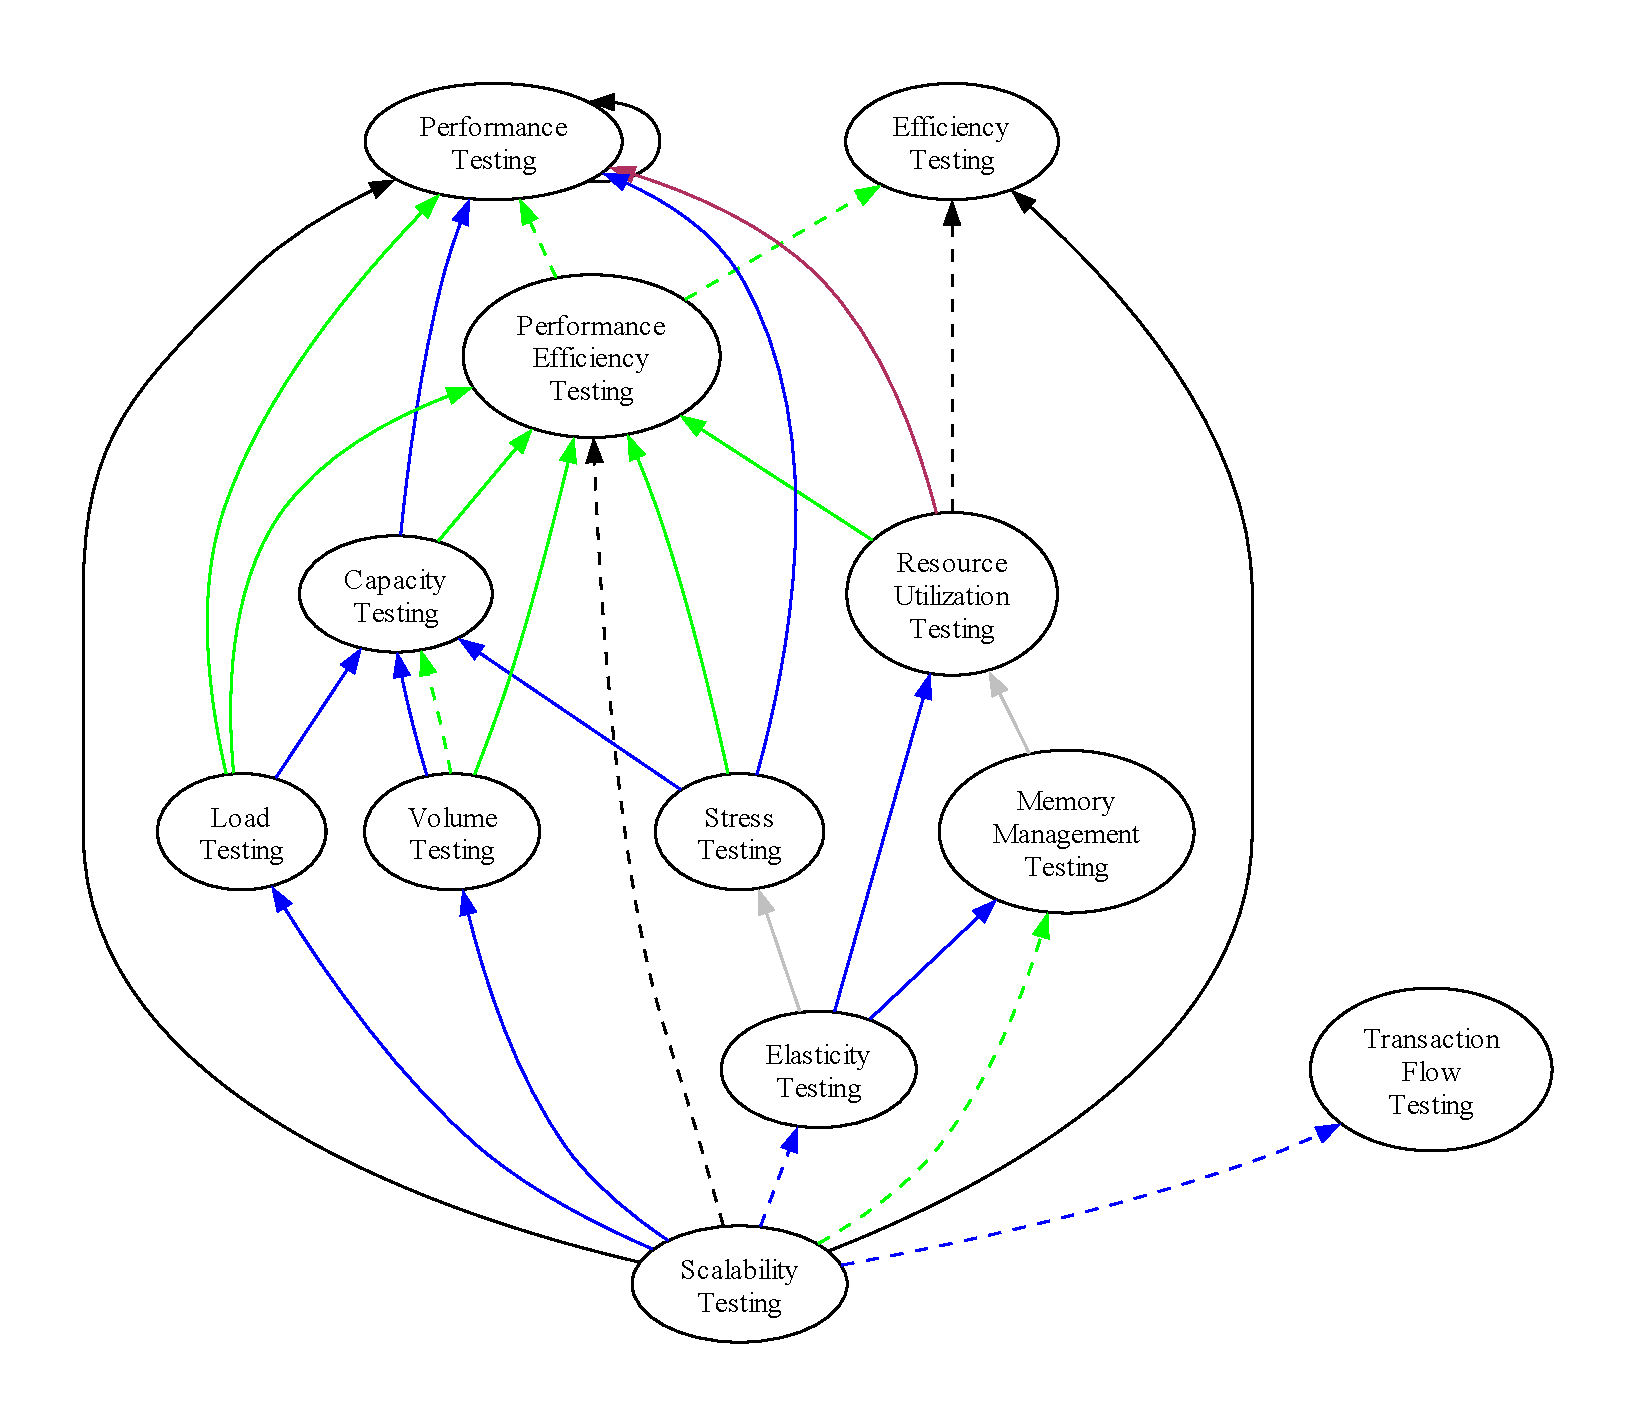
\includegraphics[width=\linewidth]{assets/graphs/scalabilityProposedGraph.pdf}
            \caption{Graph of proposed \ifnotpaper \else \\ \fi relations.}
            \label{fig:scal-graph-proposed}
        \end{subfigure}
        \caption{Graphs of relations between terms related to scalability testing.}
        \label{fig:scalGraphs}
    \end{figure}
}

\newcommand{\performanceGraph}{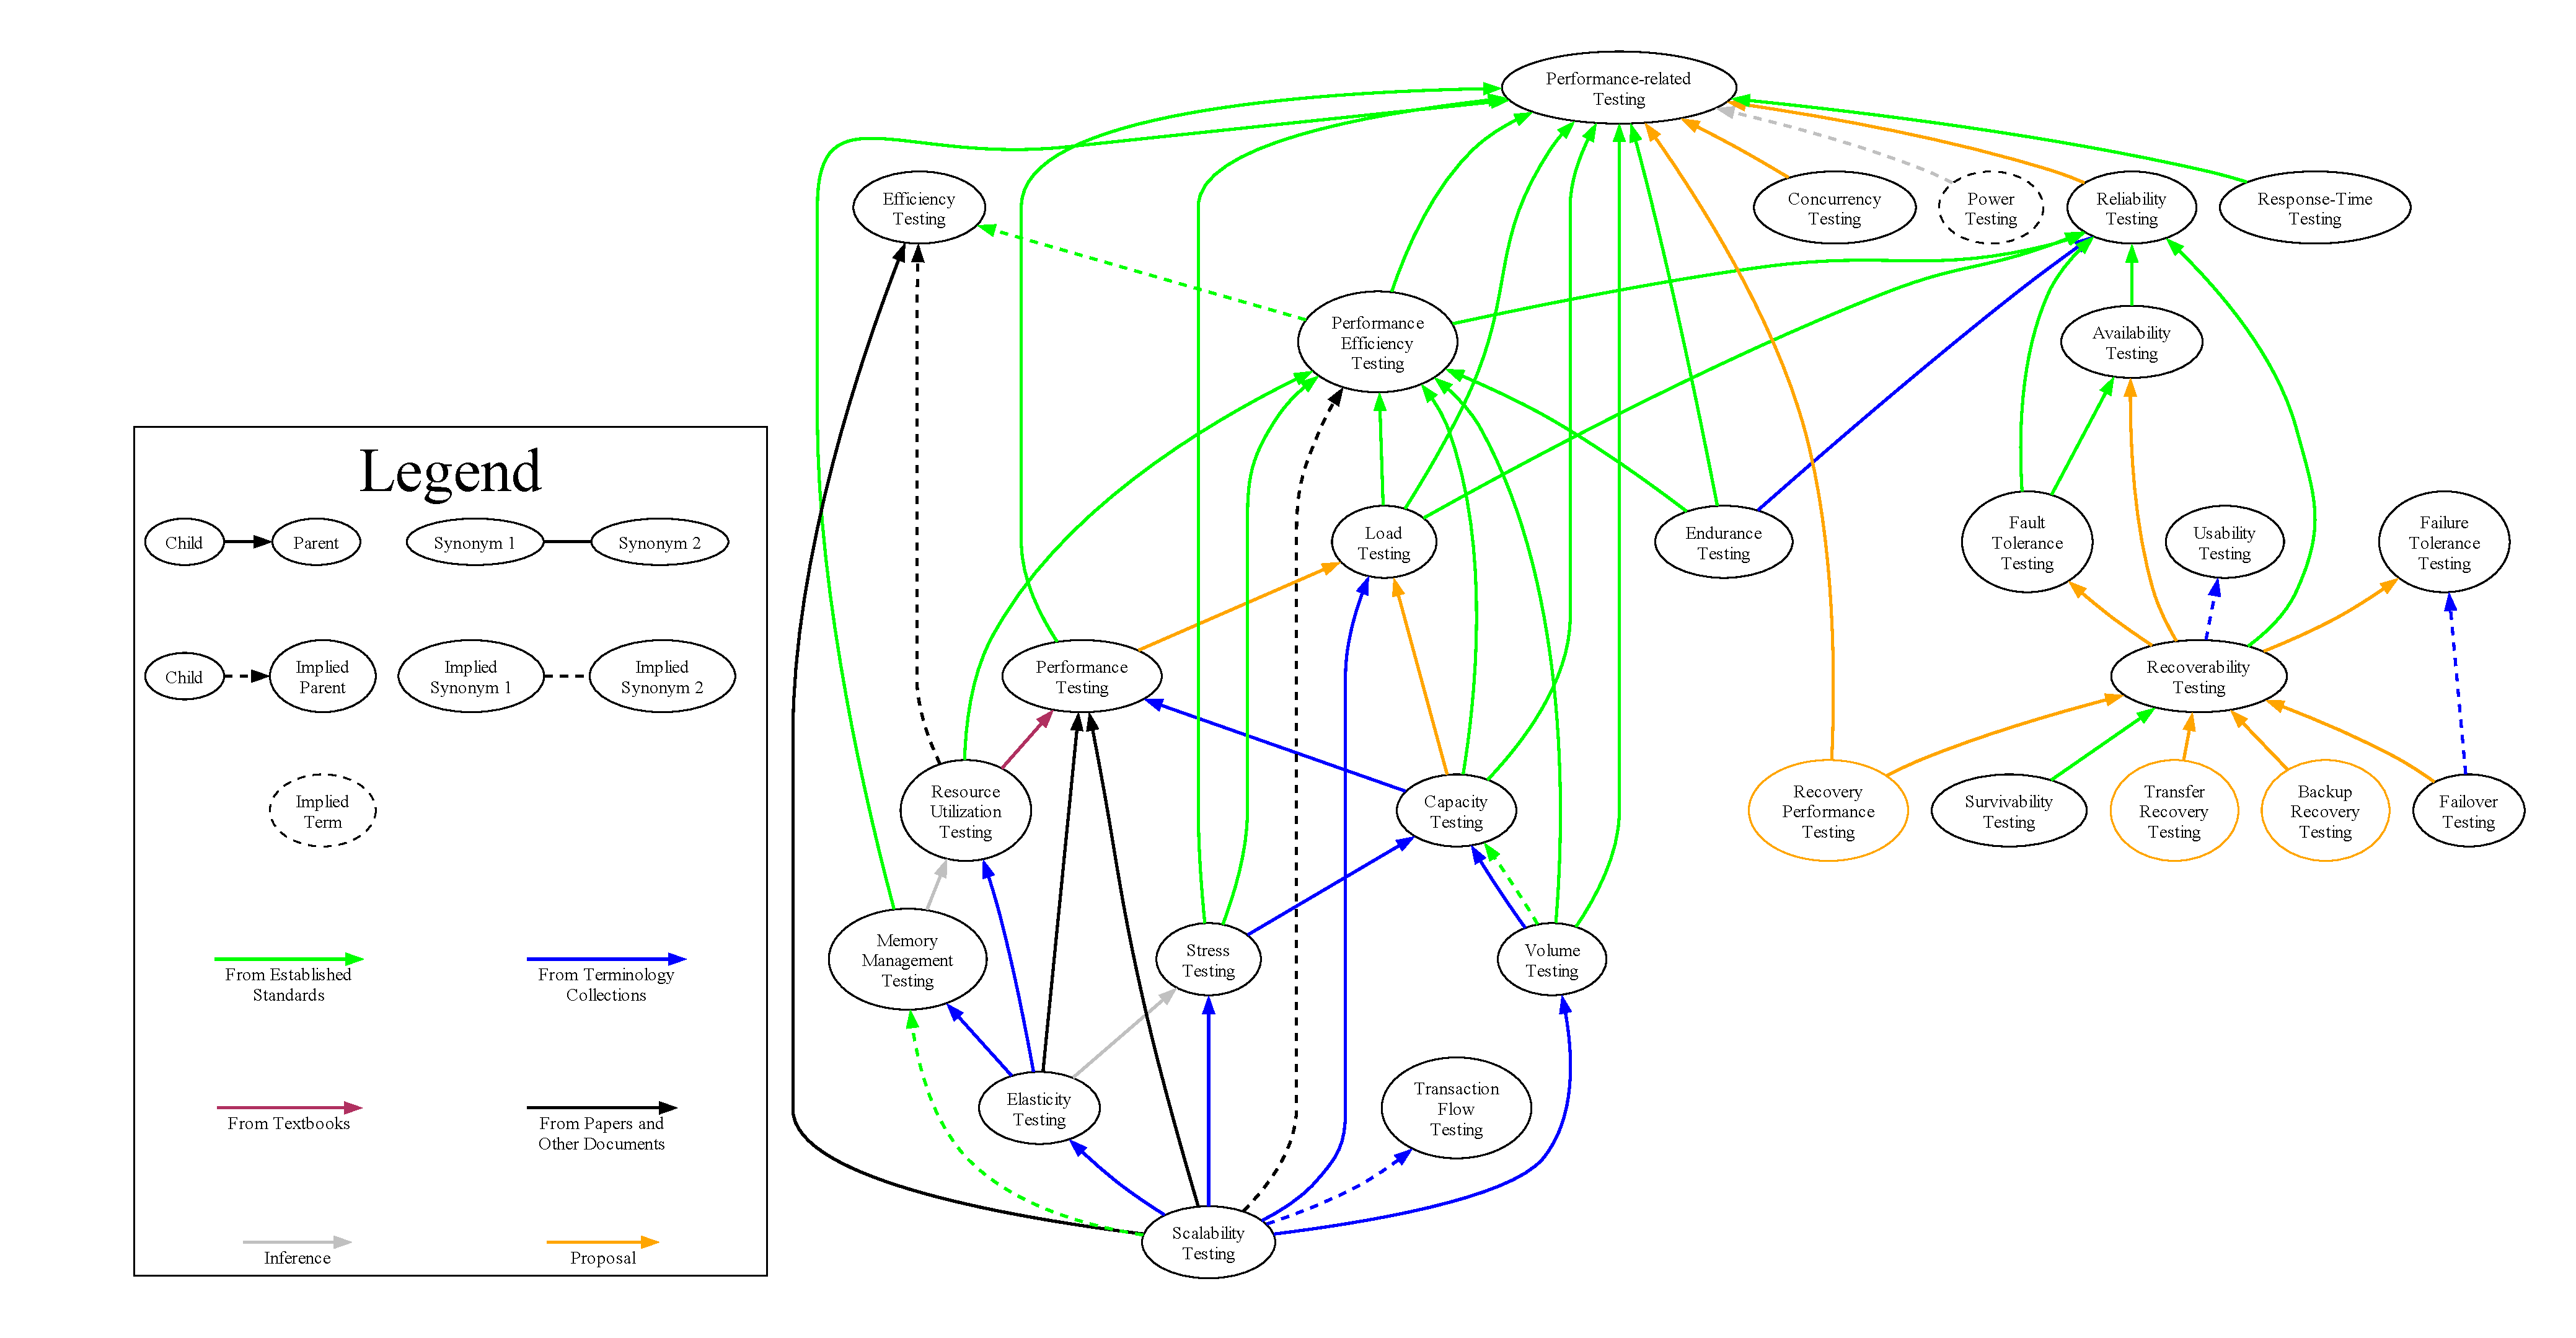
\includegraphics[width=\linewidth]{assets/graphs/performanceProposedGraph.pdf}}

%------------------------------------------------------------------------------
% Images & Figures
%------------------------------------------------------------------------------

\newcommand{\drasilLogo}{assets/images/drasil_logo.png}
\newcommand{\drasilLogoImg}{\input{assets/images/drasil_logo}}
\newcommand{\refDrasilLogoImg}{\Cref{fig:drasilLogo}}

%------------------------------------------------------------------------------
% Tables
%------------------------------------------------------------------------------

% Organization of files
\newcommand{\organizationTable}{\input{assets/tables/organization}}

\newcommand{\ieeeCatsTable}{% Conversion to (longtblr) talltblr assisted by GitHub Copilot

\begin{center}
    \begin{talltblr}[
        note{a} = {Also called ``test phase'' \ifnotpaper (see
                \flawref{level-phase-syns}) \fi or ``test stage'' \ifnotpaper
                (see \flawref{stage-level-syns})\else (see relevant synonym
                flaws in \Cref{syns})\fi.},
        note{b} = {Also called ``test design technique'' \ifnotpaper
                (\citealp[p.~11]{IEEE2022}; \citeyear[p.~5]{IEEE2021a};
                \citealpISTQB{})\else \cite[p.~11]{IEEE2022},
                \cite[p.~5]{IEEE2021a}, \cite{ISTQB}\fi.},
        caption={Categories of test approaches given by ISO/IEC and IEEE.},
        label={tab:ieeeCats}
        ]{
        colspec={|X[0.09,c,m]X[0.575,m]X[0.285,m]|},
        width = \linewidth, rowhead = 1, hlines
        }
        \thead{Term}               & \thead{Definition}                           & \thead{Examples} \\
        Test Level\TblrNote{a}     & A stage of testing ``typically associated
        with the achievement of particular objectives and used to treat particular
        risks'', each performed in sequence \ifnotpaper (\citealp[p.~12]{IEEE2022};
        \citeyear[p.~6]{IEEE2021b}) \else \cite[p.~12]{IEEE2022}, \cite[p.~6]{IEEE2021b}
        \fi with their ``own documentation and resources''
        \citeyearpar[p.~469]{IEEE2017} % ; more generally, ``designat[es] \dots\ the
        % coverage and detail'' \citeyearpar[p.~249]{IEEE2017} 
                                   & unit/component testing, integration testing,
        system testing, acceptance testing \ifnotpaper (\citeyear[p.~12]{IEEE2022};
        \citeyear[p.~6]{IEEE2021b}; \citeyear[p.~467]{IEEE2017}) \else
        \cite[p.~467]{IEEE2017}, \cite[p.~12]{IEEE2022}, \cite[p.~6]{IEEE2021b} \fi                  \\
        Test Practice              & A ``conceptual framework that can be
        applied to \dots{} [a] test process to facilitate testing'' \ifnotpaper
        (\citeyear[p.~14]{IEEE2022}; \citeyear[p.~471]{IEEE2017}; OG IEEE 2013)
        \else \cite[p.~471]{IEEE2017}, \cite[p.~14]{IEEE2022}
        \fi % ; more generally, a ``specific type of activity that contributes to
        % the execution of a process'' \citeyearpar[p.~331]{IEEE2017} 
                                   & scripted testing, exploratory testing,
        automated testing \citeyearpar[p.~20]{IEEE2022}                                              \\
        Test Technique\TblrNote{b} & A ``procedure used to create or select a
        test model \dots, identify test coverage items \dots, and derive
        corresponding test cases'' \ifnotpaper (\citeyear[p.~11]{IEEE2022};
        \citeyear[p.~5]{IEEE2021a}; similar in citeyear[p.~467]{IEEE2017}; OG
        \citeyear{IEEE2013}) \else \cite[p.~11]{IEEE2022}, \cite[p.~5]{IEEE2021a} (similar in
        \cite[p.~467]{IEEE2017}) \fi that ``generate evidence that test item
        requirements have been met or that defects are present in a test item''
        \citeyearpar[p.~vii]{IEEE2021b} ``typically used to achieve a required
        level of coverage'' \citeyearpar[p.~5]{IEEE2021a}
        % ; ``a variety \dots\ is typically
        % required to suitably cover any system'' \citeyearpar[p.~33]{IEEE2022} and
        % is ``often selected based on team skills and familiarity, on the format
        % of the test basis'', and on expectations \citeyearpar[p.~23]{IEEE2022}
                                   & equivalence partitioning,
        boundary value analysis, branch testing \ifnotpaper (\citeyear[p.~11]{IEEE2022};
        \citeyear[p.~5]{IEEE2021a}) \else \cite[p.~11]{IEEE2022}, \cite[p.~5]{IEEE2021a} \fi         \\
        Test Type                  & ``Testing that is focused on specific
        quality characteristics'' \ifnotpaper (\citeyear[p.~15]{IEEE2022};
        \citeyear[p.~7]{IEEE2021b}; \citeyear[p.~473]{IEEE2017}; OG IEEE 2013)
        \else \cite[p.~473]{IEEE2017}, \cite[p.~15]{IEEE2022}, \cite[p.~7]{IEEE2021b}
        \fi                        & security testing, usability testing,
        performance testing \ifnotpaper (\citeyear[p.~15]{IEEE2022};
        \citeyear[p.~8]{IEEE2021a}; \citeyear[p.~473]{IEEE2017}) \else
        \cite[p.~473]{IEEE2017}, \cite[p.~15]{IEEE2022}, \citeyear[p.~8]{IEEE2021a} \fi              \\
    \end{talltblr}
\end{center}
}
\newcommand{\otherCatsTable}{% Defined here so VS Code doesn't freak out
\def\ieeeEquiv{\makecell{IEEE\\Equivalent}}
\def\swebokLevel{{Level\\(objective-\\based)\TblrNote{a}}}

\begin{longtblr}[
    note{a} = {See \flawref{stage-level-syns}.},
    note{b} = {Testing methods and guidances are omitted from this table
            since \citet{BarbosaEtAl2006} do not define or give examples of them.},
    note{c} = {Synonyms for these examples are used by
            \citet[p.~3; OG Mathur, 2012]{SouzaEtAl2017} and
            \citet[p.~3]{BarbosaEtAl2006}.},
    caption={Categories of testing given by other sources.},
    label={tab:otherCats}
    ]{
    colspec={|X[0.08,c,m]|X[0.43,m]|X[0.34,m]|Q[c,m]|},
    width = \linewidth, rowhead = 1
    }
    \hline
    \thead{Term}                           & \thead{Definition}                               & \thead{Examples} & \thead{\ieeeEquiv{}} \\
    \hline
    % Guidance                               & none given
    % \citep[p.~3]{BarbosaEtAl2006}          & none given         & Technique?                              \\
    \swebokLevel{}                         & Test levels based on the
    purpose of testing \citep[p.~5\=/6]{SWEBOK2024} that ``determine
    how the test suite is identified \dots\ regarding its consistency
    \dots\ and its composition''
    \citetext{p.~5\=/2}                    & conformance testing,
    installation testing, regression testing, performance testing,
    security testing % reliability testing,
    \citep[pp.~5\=/7 to 5\=/9]{SWEBOK2024} & Type                                                                                       \\
    % Method                                 & none given
    % \citep[p.~3]{BarbosaEtAl2006}          & none given         & Practice?                               \\
    Phase                                  & none given by \citet{Perry2006} or
    \citet{BarbosaEtAl2006}
    %(\citealp[p.~221]{Perry2006}; \citealp[p.~3]{BarbosaEtAl2006})  
                                           & unit testing,
    integration testing, system testing, regression testing (\citealp[p.~221]{Perry2006};
    \citealp[p.~3]{BarbosaEtAl2006})       & Level                                                                                      \\
    Procedure                              & The basis for how
    testing is performed that guides the process; ``categorized in [to] testing methods,
    testing guidances\TblrNote{b} and testing techniques''
    \citep[p.~3]{BarbosaEtAl2006}          & none given generally by \citet{BarbosaEtAl2006};
    see ``Technique''                      & Approach                                                                                   \\
    Process                                & ``A sequence of
    testing steps'' \citep[p.~2]{BarbosaEtAl2006} ``based on a development technology and \dots\
    paradigm, as well as on a testing procedure''
    \citetext{p.~3}                        & none given by \citet{BarbosaEtAl2006}            & Practice                                \\
    Stage                                  & An
    alternative to the ``traditional \dots\ test stages'' %\footnote{See ``Level'' in \Cref{tab:ieeeCats}.}
    based on ``clear technical groupings''
    \citep[p.~13]{Gerrard2000a}            & desktop development testing,
    infrastructure testing,
    % system testing, large scale integration, and
    post-deployment monitoring
    \citep[p.~13]{Gerrard2000a}            & Level                                                                                      \\
    Technique                              & ``Systematic
    procedures and approaches for generating or selecting the most suitable test suites''
    \citep[p.~5\=/10]{SWEBOK2024}          & specification-based testing,
    % ``on a sound theoretical basis'' \citep[p.~3]{BarbosaEtAl2006}
    structure-based testing, fault-based testing\TblrNote{c}
    % , experience-based testing, usage-based testing
    (\citealp[pp.~5\=/10, 5\=/13 to 5\=/15]{SWEBOK2024})
    % black-box, white-box, defect/fault-based, model-based testing
    % \citetext{\citealp[p.~3]{SouzaEtAl2017}; OG Mathur, 2012};
    % functional, structural, error-based, state-based testing \citep[p.~3]{BarbosaEtAl2006}
                                           & Technique                                                                                  \\
    \hline
\end{longtblr}
}
\newcommand{\otherCategorizationsTable}{\def\visibExs{Specification-based Testing\\ Structure-based Testing\\ Grey-Box Testing}
\def\selecExs{Deterministic Testing\\ Random Testing}
\def\infoSrcExs{Specification-based Testing\\ Structure-based Testing\\
    Experience-based Testing\TblrNote{b}}
\def\apprExs{Specification-based Testing\\ Structure-based Testing\\ (Stepwise) Code Reading}
\def\covCritExs{Input Space Partitioning\\ Graph Coverage\\ Logic Coverage\\ Syntax-based Testing}
\def\questBase{Question Answered: What? When? Where? Who? Why? How? How Well? \citep[p.~17]{Firesmith2015}}
\def\questExs{System Testing\\ Model-based Testing\\ Scenario Testing\TblrNote{C}}
% Pair Testing\\ Unscripted Testing
\def\sdlcExs{Waterfall Testing\\ Incremental Testing\\ \acf{ct}}
\def\reasExs{Smoke Testing\\ Initial Testing\\ Regression Testing}
% Reuse Testing\\ Retesting\\ Error Seeding
\def\execExs{Static Testing\\ Dynamic Testing}
\def\goalExs{Verification Testing\\ Validation Testing}
\def\propExs{Functional Testing\\ Non-functional Testing}
\def\humInvExs{Manual Testing\\ Automated Testing}
\def\humInvCats{Practice \citep[p.~22]{IEEE2022}\\ Technique (see \Cref{tab:multiCats})}
% \citep[implied by][p.~35; see \Cref{tab:multiCats}]{IEEE2022}}
\def\strExs{Scripted Testing\\ Exploratory Testing\TblrNote{f}}
\def\covReqExs{Data Flow Testing\\ Control Flow Testing}
\def\factExs{Correctness Testing\\ Response-Time Testing\\ Access Control Testing\\
    Compliance Testing\\ Reliability Testing\\ Maintainability Testing\\ Portability Testing\\
    Performance Testing\TblrNote{e}}
\def\dataSrcExs{Specification-based Testing\\ Implementation-oriented Testing\\ Error-oriented Testing}
\def\adqCritExs{Coverage-based Testing\\ Fault-based Testing\\ Error-based Testing}
\def\typeCatExs{Static Testing\\ Test Browsing\\ Functional Testing\\
    Non-functional Testing\\ Large Scale Integration (Testing)}
\def\priorExs{Smoke Testing\\ Usability Testing\\ Performance Testing\\ Functionality Testing}
\def\purpExs{Correctness Testing\\ Performance Testing\\ Reliability Testing\\ Security Testing}

\newcommand\firesmithSubset[1]{\citep[p.~#1]{Firesmith2015}\TblrNote{d}}

\begin{longtblr}[
    note{a} = {Defined in \Cref{par-chd-rels}.},
    note{b} = {\citet[p.~440]{PetersAndPedrycz2000} replace the latter two with
            ``implementation-oriented testing'' and ``error-oriented testing''.},
    note{c} = {Experience-based testing may instead be a ``practice'' (see \Cref{tab:multiCats}).},
    % note{C} = {This list is \emph{quite} nonexhaustive.},
    note{d} = {We only present a subset of the test bases and example approaches from
            \citep{Firesmith2015} for brevity.},
    note{e} = {We also consider this categorization meaningful (see \Cref{static-test}).},
    % note{e} = {Other test factors are given that do not unambiguously map to corresponding
    %         test approaches: file integrity, authorization, audit trail, continuity of processing,
    %         service levels, ease of use, coupling (e.g., with other applications in a given environment),
    %         and ease of operation (e.g., documentation, training) \citep[pp.~40--41]{Perry2006}.},
    note{f} = {This grouping is likely incorrect (see \Cref{exp-unscrip}).},
    note{g} = {Exploratory testing may instead be a ``technique'' (see \Cref{tab:multiCats}).},
    note{h} = {\citet[p.~49]{Firesmith2015} less-than-helpfully calls this basis ``whitebox testing''.},
    note{i} = \gerrardDistinctIEEE*{type},
    note{j} = {With the exception of smoke testing, which is categorized as a technique
            (\citealp[p.~5\=/14]{SWEBOK2024}; \citealp[pp.~601, 603, 605--606]{SharmaEtAl2021});
            performance testing is also sometimes categorized as a technique \citep[p.~38]{IEEE2021}.},
    caption = {Alternate categorizations found in the literature.},
    label = {tab:otherCategorizations}
    ]{
    colspec = {|X[0.375,c,m]X[0.275,c,m]X[0.35,c,m]|},
    width = \linewidth, rowhead = 1
    }
    \hline
    \thead{Test Basis}                      & \thead{Example Approaches} & \thead{Parent\TblrNote{a} IEEE Category}                                                                                                 \\
    \hline
    Visibility of the \acs{sut}'s Internal Structure (\citealp[p.~8]{IEEE2021};
    \citealp[pp.~5\=/10, 5\=/16]{SWEBOK2024};
    % \citealp[pp.~53, 218]{Patton2006}; \citealp[p.~69]{Perry2006}; \citealp[p.~601; OG {[8]}]{SharmaEtAl2021};
    % \citealp[pp.~57--58]{AmmannAndOffutt2017}; \citealp[p.~213]{KuļešovsEtAl2013}; \citep[pp.~4--5]{Kam2008}
    six other sources)                      & \visibExs{}                & Technique (\citealp[pp.~4, 8]{IEEE2021}; \citealp[p.~46]{Firesmith2015})                                                                 \\
    \hline
    Source of Information for Designing Tests
    \citep[p.~8; one more source]{IEEE2021} & \infoSrcExs{}              & Technique\TblrNote{c} (\citealp[p.~22]{IEEE2022}; \citeyear[p.~4]{IEEE2021}; three other sources)                                        \\
    % & & \citealp[pp.~5\=/10, 5\=/13]{SWEBOK2024}; \citealpISTQB{}; \citealp[p.~46]{Firesmith2015}) \\
    \hline
    % Source of Test Data
    % \citep[p.~440]{PetersAndPedrycz2000}    & \dataSrcExs{}              & Technique                                                                                                                                \\
    % \hline
    Selection Process
    \citep[p.~5-16]{SWEBOK2024}             & \selecExs{}                & Technique \citep[pp.~5\=/12, 5\=/16]{SWEBOK2024}                                                                                         \\
    \hline
    % \questBase{}                             & \questExs{}                & Approach                                                                                                                                                               \\
    % \hline
    Stage of Lifecycle \firesmithSubset{29} & \sdlcExs{}                 & Practice                                                                                                                                 \\
    \hline
    Reason \firesmithSubset{34}             & \reasExs{}                 & Technique                                                                                                                                \\
    \hline
    Level of Automation \firesmithSubset{44;
        % \citep[p.~214]{KuļešovsEtAl2013}
    one other source}                       & \humInvExs{}               & \humInvCats{}                                                                                                                            \\
    \hline
    Execution of Code\TblrNote{e} \citep[p.~53; two other sources]{Patton2006}
    % \citealp[p.~214]{KuļešovsEtAl2013}; \citealp[p.~12]{Gerrard2000a}
                                            & \execExs{}                 & Approach                                                                                                                                 \\
    \hline
    Goal \citep[pp.~69--70; one other source]{Perry2006};
    % \citealp[p.~214]{KuļešovsEtAl2013}
                                            & \goalExs{}                 & Approach                                                                                                                                 \\
    \hline
    % Seems synonymous with testing based on software qualities
    % Test Factor (also called Quality Factor or Quality Attribute)
    % \citep[pp.~40--41]{Perry2006}           & \factExs{}                 & Type (\citealp[p.~22]{IEEE2022}; and/or implied by its quality and/or \citealp{Firesmith2015})                                           \\
    % \hline
    Adequacy Criterion
    \citep[pp.~398--399]{vanVliet2000}      & \adqCritExs{}              & Technique \citep[pp.~398--399]{vanVliet2000}                                                                                             \\
    \hline
    Coverage Criteria
    \citep[pp.~18--19]{AmmannAndOffutt2017} & \covCritExs{}              & Technique (\citealp[p.~22]{IEEE2022}; \citeyear[Fig.~2]{IEEE2021}; \citealp[p.~5\=/11]{SWEBOK2024}; \citealp[pp.~47--48]{Firesmith2015}) \\
    \hline
    Structuredness
    \citep[p.~214]{KuļešovsEtAl2013}        & \strExs{}                  & Practice\TblrNote{g} \citep[pp.~20, 22]{IEEE2022}                                                                                        \\
    \hline
    Property of Code \citep[p.~213]{KuļešovsEtAl2013}
    or Test Target
    \citep[pp.~4--5]{Kam2008}               & \propExs{}                 & Ambiguous (see \Cref{func-test-flaw})                                                                                                    \\
    \hline
    Coverage Requirement\TblrNote{h}
    \citep[pp.~4--5]{Kam2008}               & \covReqExs{}               & Technique (\citealp[p.~5\=/13]{SWEBOK2024}; \citealp[p.~49]{Firesmith2015})                                                              \\
    \hline
    Category of Test Type\TblrNote{i}
    \citep[p.~12]{Gerrard2000a}             & \typeCatExs{}              & Ambiguous                                                                                                                                \\
    \hline
    Priority (in the context of testing e-business projects)
    \citep[p.~13]{Gerrard2000a}             & \priorExs{}                & Type\TblrNote{j} (\citealp[p.~22]{IEEE2022}; \citeyear[Tab.~A.1]{IEEE2021}; and/or implied by \citealp[p.~53]{Firesmith2015})            \\
    \hline
    Purpose \citep{Pan1999}                 & \purpExs{}                 & Type (\citealp[p.~22]{IEEE2022}; and/or implied by \citealp[p.~53]{Firesmith2015})                                                       \\
    \hline
\end{longtblr}
}

\newcommand{\flawMnfstsTable}{\begin{paperTable}
    \centering
    \caption{Breakdown of identified \nameref{flawMnfsts} by \srcCat{}.}
    \label{tab:flawMnfsts}
    \begin{minipage}{\linewidth}
        \begin{tabular}{|r|*{6}{cc|}c|}
            \hline
                              & \multicolumn{2}{c|}{\thead{\wrong{}}} & \multicolumn{2}{c|}{\thead{\miss{}}} & \multicolumn{2}{c|}{\thead{\contra{}}} & \multicolumn{2}{c|}{\thead{\ambi{}}} & \multicolumn{2}{c|}{\thead{\over{}}} & \multicolumn{2}{c|}{\thead{\redun{}}} &                                                                                                                                                                                                \\
            \thead{\srcCat{}} & \thead{Exp}                           & \thead{Imp}                          & \thead{Exp}                            & \thead{Imp}                          & \thead{Exp}                          & \thead{Imp}                           & \thead{Exp}              & \thead{Imp}              & \thead{Exp}              & \thead{Imp}               & \thead{Exp}               & \thead{Imp}               & \thead{Total}             \\
            \hline
            \stds{}           & \stdFlawMnfstBrkdwn{1}                & \stdFlawMnfstBrkdwn{2}               & \stdFlawMnfstBrkdwn{3}                 & \stdFlawMnfstBrkdwn{4}               & \stdFlawMnfstBrkdwn{5}               & \stdFlawMnfstBrkdwn{6}                & \stdFlawMnfstBrkdwn{7}   & \stdFlawMnfstBrkdwn{8}   & \stdFlawMnfstBrkdwn{9}   & \stdFlawMnfstBrkdwn{10}   & \stdFlawMnfstBrkdwn{11}   & \stdFlawMnfstBrkdwn{12}   & \stdFlawMnfstBrkdwn{13}   \\
            \metas{}          & \metaFlawMnfstBrkdwn{1}               & \metaFlawMnfstBrkdwn{2}              & \metaFlawMnfstBrkdwn{3}                & \metaFlawMnfstBrkdwn{4}              & \metaFlawMnfstBrkdwn{5}              & \metaFlawMnfstBrkdwn{6}               & \metaFlawMnfstBrkdwn{7}  & \metaFlawMnfstBrkdwn{8}  & \metaFlawMnfstBrkdwn{9}  & \metaFlawMnfstBrkdwn{10}  & \metaFlawMnfstBrkdwn{11}  & \metaFlawMnfstBrkdwn{12}  & \metaFlawMnfstBrkdwn{13}  \\
            \texts{}          & \textFlawMnfstBrkdwn{1}               & \textFlawMnfstBrkdwn{2}              & \textFlawMnfstBrkdwn{3}                & \textFlawMnfstBrkdwn{4}              & \textFlawMnfstBrkdwn{5}              & \textFlawMnfstBrkdwn{6}               & \textFlawMnfstBrkdwn{7}  & \textFlawMnfstBrkdwn{8}  & \textFlawMnfstBrkdwn{9}  & \textFlawMnfstBrkdwn{10}  & \textFlawMnfstBrkdwn{11}  & \textFlawMnfstBrkdwn{12}  & \textFlawMnfstBrkdwn{13}  \\
            \papers*{}        & \paperFlawMnfstBrkdwn{1}              & \paperFlawMnfstBrkdwn{2}             & \paperFlawMnfstBrkdwn{3}               & \paperFlawMnfstBrkdwn{4}             & \paperFlawMnfstBrkdwn{5}             & \paperFlawMnfstBrkdwn{6}              & \paperFlawMnfstBrkdwn{7} & \paperFlawMnfstBrkdwn{8} & \paperFlawMnfstBrkdwn{9} & \paperFlawMnfstBrkdwn{10} & \paperFlawMnfstBrkdwn{11} & \paperFlawMnfstBrkdwn{12} & \paperFlawMnfstBrkdwn{13} \\
            \hline
            Total             & \totalFlawMnfstBrkdwn{1}              & \totalFlawMnfstBrkdwn{2}             & \totalFlawMnfstBrkdwn{3}               & \totalFlawMnfstBrkdwn{4}             & \totalFlawMnfstBrkdwn{5}             & \totalFlawMnfstBrkdwn{6}              & \totalFlawMnfstBrkdwn{7} & \totalFlawMnfstBrkdwn{8} & \totalFlawMnfstBrkdwn{9} & \totalFlawMnfstBrkdwn{10} & \totalFlawMnfstBrkdwn{11} & \totalFlawMnfstBrkdwn{12} & \totalFlawMnfstBrkdwn{13} \\
            \hline
        \end{tabular}
    \end{minipage}
\end{paperTable}
}
\newcommand{\flawDmnsTable}{\begin{paperTable}
    \centering
    \caption{Breakdown of identified \nameref{flawDmns} by \srcCat{}.}
    \label{tab:flawDmns}
    % \begin{minipage}{\linewidth}
    \begin{tabular}{|r|*{6}{cc|}c|}
        \hline
                          & \multicolumn{2}{c|}{\thead{\cats{}}} & \multicolumn{2}{c|}{\thead{\syns{}}} & \multicolumn{2}{c|}{\thead{\pars{}}} & \multicolumn{2}{c|}{\thead{\defs{}}} & \multicolumn{2}{c|}{\thead{\terms{}}} & \multicolumn{2}{c|}{\thead{\cites{}}} &                                                                                                                                                                                  \\
        % \cline{2-10}
        \thead{\srcCat{}} & \thead{Exp}                          & \thead{Imp}                          & \thead{Exp}                          & \thead{Imp}                          & \thead{Exp}                           & \thead{Imp}                           & \thead{Exp}            & \thead{Imp}            & \thead{Exp}            & \thead{Imp}             & \thead{Exp}             & \thead{Imp}             & \thead{Total}           \\
        \hline
        \stds{}           & \stdFlawDmnBrkdwn{1}                 & \stdFlawDmnBrkdwn{2}                 & \stdFlawDmnBrkdwn{3}                 & \stdFlawDmnBrkdwn{4}                 & \stdFlawDmnBrkdwn{5}                  & \stdFlawDmnBrkdwn{6}                  & \stdFlawDmnBrkdwn{7}   & \stdFlawDmnBrkdwn{8}   & \stdFlawDmnBrkdwn{9}   & \stdFlawDmnBrkdwn{10}   & \stdFlawDmnBrkdwn{11}   & \stdFlawDmnBrkdwn{12}   & \stdFlawDmnBrkdwn{13}   \\
        \metas{}          & \metaFlawDmnBrkdwn{1}                & \metaFlawDmnBrkdwn{2}                & \metaFlawDmnBrkdwn{3}                & \metaFlawDmnBrkdwn{4}                & \metaFlawDmnBrkdwn{5}                 & \metaFlawDmnBrkdwn{6}                 & \metaFlawDmnBrkdwn{7}  & \metaFlawDmnBrkdwn{8}  & \metaFlawDmnBrkdwn{9}  & \metaFlawDmnBrkdwn{10}  & \metaFlawDmnBrkdwn{11}  & \metaFlawDmnBrkdwn{12}  & \metaFlawDmnBrkdwn{13}  \\
        \texts{}          & \textFlawDmnBrkdwn{1}                & \textFlawDmnBrkdwn{2}                & \textFlawDmnBrkdwn{3}                & \textFlawDmnBrkdwn{4}                & \textFlawDmnBrkdwn{5}                 & \textFlawDmnBrkdwn{6}                 & \textFlawDmnBrkdwn{7}  & \textFlawDmnBrkdwn{8}  & \textFlawDmnBrkdwn{9}  & \textFlawDmnBrkdwn{10}  & \textFlawDmnBrkdwn{11}  & \textFlawDmnBrkdwn{12}  & \textFlawDmnBrkdwn{13}  \\
        \papersTbl{}      & \paperFlawDmnBrkdwn{1}               & \paperFlawDmnBrkdwn{2}               & \paperFlawDmnBrkdwn{3}               & \paperFlawDmnBrkdwn{4}               & \paperFlawDmnBrkdwn{5}                & \paperFlawDmnBrkdwn{6}                & \paperFlawDmnBrkdwn{7} & \paperFlawDmnBrkdwn{8} & \paperFlawDmnBrkdwn{9} & \paperFlawDmnBrkdwn{10} & \paperFlawDmnBrkdwn{11} & \paperFlawDmnBrkdwn{12} & \paperFlawDmnBrkdwn{13} \\
        \hline
        Total             & \totalFlawDmnBrkdwn{1}               & \totalFlawDmnBrkdwn{2}               & \totalFlawDmnBrkdwn{3}               & \totalFlawDmnBrkdwn{4}               & \totalFlawDmnBrkdwn{5}                & \totalFlawDmnBrkdwn{6}                & \totalFlawDmnBrkdwn{7} & \totalFlawDmnBrkdwn{8} & \totalFlawDmnBrkdwn{9} & \totalFlawDmnBrkdwn{10} & \totalFlawDmnBrkdwn{11} & \totalFlawDmnBrkdwn{12} & \totalFlawDmnBrkdwn{13} \\
        \hline
    \end{tabular}
    % \end{minipage}
\end{paperTable}}

\newcommand{\testReqsTable}{\input{assets/tables/testReqs}}

\notpapertrue

\newenvironment{paperTable}{
    \begingroup
    \renewcommand*{\thefootnote}{\alph{footnote}}
    \begin{table}[hbtp!]
        }{
    \end{table}
    \endgroup
}

\renewcommand\stds{\stdSources{1}}
\renewcommand\metas{\metaSources{1}}
\renewcommand\texts{\textSources{1}}
\renewcommand\papers{\paperSources{1}}

\newcounter{methodCounter}

\title[Committee Meeting 2]{Second Committee Meeting}
\subtitle{Updated Progress Report}
\author{\thesisAuthorName{}}

% Committee
% \begin{itemize}
%     \item \emph{Supervisor}: Dr.~Jacques Carette
%     \item \emph{Supervisor}: Dr.~Spencer Smith
%     \item Dr.~Ned Nedialkov
%     \item Dr.~Richard Paige
% \end{itemize}

\institute{McMaster University}
\date{Fall 2025}

\AtBeginSection[]
{
  \begin{frame}
    \frametitle{Table of Contents}
    \tableofcontents[currentsection]
  \end{frame}
}

\begin{document}

% From https://tex.stackexchange.com/a/42826/192195
\NewDocumentCommand{\ShowListingForLineNumber}{s O{1.0} m m}{
    \IfBooleanTF{#1}{\vspace{-#2\baselineskip}}{}
    \lstinputlisting[
        style=MyListStyle,
        linerange={#3-#3},
        firstnumber=#3,
    ]{#4}
}

%%%%%%%%%%%%%%%%%%%%%%%%%%%%%%%%%%%%%%%%%%%%%%%%%%%%%%%%%%%%%%%%%%%%%%%%%%%%%%%
%% TITLE PAGE
%%%%%%%%%%%%%%%%%%%%%%%%%%%%%%%%%%%%%%%%%%%%%%%%%%%%%%%%%%%%%%%%%%%%%%%%%%%%%%%
\frame{\titlepage}

%%%%%%%%%%%%%%%%%%%%%%%%%%%%%%%%%%%%%%%%%%%%%%%%%%%%%%%%%%%%%%%%%%%%%%%%%%%%%%%
%% TABLE OF CONTENTS
%%%%%%%%%%%%%%%%%%%%%%%%%%%%%%%%%%%%%%%%%%%%%%%%%%%%%%%%%%%%%%%%%%%%%%%%%%%%%%%

\begin{frame}
    \frametitle{Table of Contents}
    \tableofcontents
\end{frame}

%%%%%%%%%%%%%%%%%%%%%%%%%%%%%%%%%%%%%%%%%%%%%%%%%%%%%%%%%%%%%%%%%%%%%%%%%%%%%%%
%% INTRODUCTION
%%%%%%%%%%%%%%%%%%%%%%%%%%%%%%%%%%%%%%%%%%%%%%%%%%%%%%%%%%%%%%%%%%%%%%%%%%%%%%%
\section{Introduction}

% \subsection{The Need for Standardized Terminology}

% \subsection{The Lack of Standardized Terminology}

% \begin{frame}[c]{The Lack of Standardized Terminology}
%     \framesubtitle{``The Problem''}
%     \begin{figure}
%         \centering
%         \only{\includegraphics[height=0.65\textheight]{assets/images/test approach choices}
%             \caption{\tiny \citep[Fig.~2]{IEEE2022}}}<1>
%         \only{\includegraphics[height=0.65\textheight]{assets/images/test approach exp based}
%             \caption{\tiny Adapted from \citep[Fig.~2]{IEEE2022}}}<2>
%         \only{\includegraphics[width=\textwidth]{assets/images/exp based 2}
%             \caption{\tiny Adapted from \citep[p.~34]{IEEE2022}}}<3>
%     \end{figure}
% \end{frame}

% \begin{frame}[c]{The Lack of Standardized Terminology}
%     \framesubtitle{``The Problem'' (cont.)}
%     \begin{figure}
%         \begin{center}
%             \only{\includegraphics[height=0.65\textheight]{assets/images/system testing}
%                 \caption{\tiny \citep[p.~23]{Firesmith2015}}}<1>
%             \only{\includegraphics[height=0.65\textheight]{assets/images/system testing hil}
%                 \caption{\tiny Adapted from \citep[p.~23]{Firesmith2015}}}<2>
%             \only{\includegraphics[height=0.65\textheight]{assets/images/system testing sos}
%                 \caption{\tiny Adapted from \citep[p.~23]{Firesmith2015}}}<3>
%             \only{\includegraphics[height=0.65\textheight]{assets/images/system testing self}
%                 \caption{\tiny Adapted from \citep[p.~23]{Firesmith2015}}}<4>
%             \only{\includegraphics[height=0.65\textheight]{assets/images/system testing int}
%                 \caption{\tiny Adapted from \citep[p.~23]{Firesmith2015}}}<5>
%             \only{\includegraphics[height=0.65\textheight]{assets/images/system testing int 2}
%                 \begin{columns}
%                     \centering
%                     \begin{column}{0.4\textwidth}
%                         \caption{\tiny Adapted from \citepISTQB{}}
%                     \end{column}
%                     \begin{column}{0.4\textwidth}
%                         \caption{\tiny Adapted from \citep[p.~23]{Firesmith2015}}
%                     \end{column}
%                 \end{columns}
%             }<6>
%         \end{center}
%     \end{figure}
% \end{frame}

% \begin{frame}
%     \frametitle{Barriers to Effective Communication}
%     \framesubtitle{``The Problem'' (cont.)}
%     \vspace{-1cm}
%     \begin{columns}[T]
%         \begin{column}{.5\textwidth}
%             \begin{center}
%                 \huge Interorganizational

%                 \normalsize Schools, companies, etc.

%                 \vspace{5mm}

%                 % Based on code frustratingly generated by ChatGPT
%                 \begin{tikzpicture}

%                     % Define coordinates of the triangle's vertices
%                     \coordinate (A) at (0, 0);
%                     \coordinate (B) at (3, 0);
%                     \coordinate (C) at (1.5, 2.6);
%                     \coordinate (D) at (1.5, 0.86667);

%                     % Draw circles at each vertex without labels
%                     \draw[fill=blue!20] (A) circle [radius=0.5];
%                     \draw[fill=blue!20] (B) circle [radius=0.5];
%                     \draw[fill=blue!20] (C) circle [radius=0.5];

%                     % Draw arrows as arcs
%                     \draw[->, thick, shorten <= 20pt] (B) arc (0:48:3cm);
%                     \draw[->, thick, shorten <= 20pt] (C) arc (120:168:3cm);
%                     \draw[->, thick, shorten <= 20pt] (A) arc (240:288:3cm);

%                     % Small diagrams inside each circle
%                     \only<2->{
%                         \foreach \x in {A,B,C} {
%                                 \begin{scope}[shift={(\x)}, scale=0.2] % Scaling down and shifting to position A
%                                     \coordinate (D) at (-1.25, -0.75);
%                                     \coordinate (E) at (1.25, -0.75);
%                                     \coordinate (F) at (0, 1.5);
%                                     \draw[fill=blue!20] (D) circle [radius=0.5];
%                                     \draw[fill=blue!20] (E) circle [radius=0.5];
%                                     \draw[fill=blue!20] (F) circle [radius=0.5];
%                                     \draw[->, shorten <= 4pt] (E) arc (0:45:2.5cm);
%                                     \draw[->, shorten <= 4pt] (F) arc (120:165:2.5cm);
%                                     \draw[->, shorten <= 4pt] (D) arc (240:285:2.5cm);
%                                 \end{scope}
%                             }
%                     }
%                 \end{tikzpicture}
%             \end{center}
%         \end{column}
%         \begin{column}<2->{.5\textwidth}
%             \begin{center}
%                 \huge Intraorganizational \normalsize
%             \end{center}

%             ``Complete testing'' could require the tester to:
%             \begin{itemize}
%                 \item discover every bug,
%                 \item exhaust the time allocated,
%                 \item implement every planned test,
%                 \item \dots{} \tiny \citep[p.~7]{KanerEtAl2011}
%                       \normalsize \hspace{0pt} % For bullet spacing
%             \end{itemize}
%         \end{column}
%     \end{columns}
% \end{frame}

%%%%%%%%%%%%%%%%%%%%%%%%%%%%%%%%%%%%%%%%%%%%%%%%%%%%%%%%%%%%%%%%%%%%%%%%%%%%%%%
%% PROJECT
%%%%%%%%%%%%%%%%%%%%%%%%%%%%%%%%%%%%%%%%%%%%%%%%%%%%%%%%%%%%%%%%%%%%%%%%%%%%%%%

\section{Project}
\subsection{Research Questions}

\def\rqa{\begin{alertblock}{Research Question 1}
        \rqatext{}
    \end{alertblock}
}

\def\rqb{\begin{alertblock}{Research Question 2}
        \rqbtext{}
    \end{alertblock}
}

\def\rqc{\begin{alertblock}{Research Question 3}
        \rqctext{}
    \end{alertblock}
}

\begin{frame}{Research Questions}
    \onslide<1->\rqa{} \vspace*{\fill}
    \onslide<1>\rqb{} \vspace*{\fill}
    \onslide<1>\rqc{} \vspace*{\fill}
    \vspace{0.2cm}
\end{frame}

\subsection{Methodology}

\input{build/methodOverviewSem}

\begin{frame}{Methodology}
    \framesubtitle{Procedure}
    \begin{itemize}
        \item We build a glossary with a row for each test approach
    \end{itemize}
    \begin{center}
        \begin{table}
            \small
            \begin{tabularx}{\linewidth}{|M{1.1cm}|M{1.3cm}|X|M{1.5cm}|M{1.6cm}|}
                \hline
                \thead{\textbf{Name}} & \thead{\textbf{Category}} & \thead{\textbf{Definition}}                                                                                         & \thead{\textbf{Parent(s)}}                       & \thead{\textbf{Synonym(s)}}           \\
                \hline
                A/B Testing           & Practice {\tiny (Fig.~2)} & Testing ``that allows testers to determine which of two systems or components performs better'' {\tiny (pp.~1, 36)} & Statistical Testing {\tiny (pp.~1,~36)}, \dots{} & Split-Run Testing {\tiny (pp.~1,~36)} \\
                \hline
            \end{tabularx}
            \caption{\tiny Information from \citep{IEEE2022}}
        \end{table}
    \end{center}
    \pause \vspace{-0.5cm}
    \begin{itemize}
        \item We gather this information from sources by looking for:
              \begin{itemize}
                  \item Glossaries, taxonomies, hierarchies, etc.
                  \item Testing-related terms
                  \item Terms described \emph{by} other approaches
                  \item Terms that \emph{imply} other approaches
              \end{itemize}
    \end{itemize}
\end{frame}

% \begin{frame}{Methodology}
%     \framesubtitle{Procedure}
%     \begin{itemize}
%         \item It seems that the existence of a software quality implies the
%               existence of a test type associated with it \pause
%         \item Some test approaches use shared or complicated terminology \pause
%         \item For each of these, we record its
%               \begin{itemize}
%                   \item Name
%                   \item Definition
%                   \item Precedence for a related test type (only for qualities)
%                   \item Synonym(s)
%               \end{itemize}
%     \end{itemize}
% \end{frame}

% \begin{frame}{Methodology}
%     \framesubtitle{Procedure}
%     \begin{itemize}
%         \item Recording these data in a consistent format allows for visualizations to
%               be generated according to a certain logic \pause
%         \item It also allows for subsets of flaws to be identified \pause
%               \vspace{1cm}\rqb{}
%     \end{itemize}
% \end{frame}

\begin{frame}{Methodology}
    \framesubtitle{Sources}
    \begin{figure}
        \centering
        \begin{tikzpicture}
            \pie[sum=auto, after number=, text=legend, thick,
                scale=\ifnotpaper0.7\else0.5\fi,
                every label/.style={align=left, scale=0.7}]
            {\stdSources{3}/\stds{},
                \metaSources{3}/\metas{},
                \textSources{3}/\texts{},
                \paperSources{3}/\papers{}}

            \onslide<1>{
                \node[anchor=west, align=center] at (0, 3) {
                    In total, we investigate \srcCount{} sources
                };
            }

            \onslide<2>{
                \node[anchor=west, align=center] at (-2.2, 3) {
                    Textbooks used at McMaster were our ad hoc starting points\\
                    \tiny \citep{Patton2006, PetersAndPedrycz2000, vanVliet2000}
                };
                \draw[->, very thick] (-1.8, 2.9) -- (-1.55, 1.1);
            }

            % \onslide<3>{
            %     \node[anchor=west, align=left] at (2.4, -2) {
            %         Includes websites \citetext{\citealp{LambdaTest2024}; \\
            %             \quad\quad\citealp{Pandey2023}} and a booklet\\
            %         \quad\quad\citep{SPICE2022}};
            %     \draw[->, very thick] (2.25, -1.5) -- (1.25, -1.1);
            % }

        \end{tikzpicture}
    \end{figure}
\end{frame}

\begin{frame}[t]{Methodology}
    \framesubtitle{Categories}
    \vspace{-0.925cm}
    \centering
    \only<1>{\includegraphics[width=\linewidth]{assets/graphs/manual/catRels1.pdf}}
    \only<2>{\includegraphics[width=\linewidth]{assets/graphs/manual/catRels2.pdf}}
    \only<3>{\includegraphics[width=\linewidth]{assets/graphs/manual/catRels3.pdf}}
    \only<4>{\includegraphics[width=\linewidth]{assets/graphs/manual/catRels4.pdf}}
    \only<5>{\includegraphics[width=\linewidth]{assets/graphs/manual/catRels5.pdf}}

    \begin{minipage}{0.98\textwidth}
        % For weird spacing issue
        \only<1-3>{\vspace{-0.8cm}}
        \only<4>{\vspace{-0.475cm}}
        \only<5>{\vspace{0.02cm}}
        \only<1>{\textbf{Approach:} a ``high-level test implementation choice''
            \citep[p.~10]{IEEE2022} used to ``pick the particular test case
            values'' \citeyearpar[p.~465]{IEEE2017}}
        \only<2>{\textbf{Level:} a stage of testing with ``particular
            objectives and \dots{} risks'', each performed in sequence
            (\citealp[p.~12]{IEEE2022}; \citeyear[p.~6]{IEEE2021a};
            \citeyear[p.~6]{IEEE2021c})}
        \only<3>{\textbf{Practice:} a ``conceptual framework that can be applied
            to \dots{} [a] test process to facilitate testing''
            (\citealp[p.~14]{IEEE2022}; \citeyear[p.~471]{IEEE2017})}
        \only<4>{\textbf{Technique:} a
            % ``defined'' and ``systematic'' \citep[p.~464]{IEEE2017}
            ``procedure used to create or select a test
            model, identify test coverage items, and derive corresponding test cases''
            (\citeyear[p.~11]{IEEE2022}; \citeyear[p.~5]{IEEE2021a};
            similar in \citeyear[p.~467]{IEEE2017})}
        \only<5>{\textbf{Type:} ``Testing that is focused on specific quality
            characteristics'' (\citealp[p.~15]{IEEE2022}; \citeyear[p.~7]{IEEE2021c};
            \citeyear[p.~473]{IEEE2017})}
    \end{minipage}
\end{frame}

\begin{frame}[t]{Methodology}
    \framesubtitle{Visualization Notation}
    \vspace{-0.925cm}
    \centering
    \only<1>{\includegraphics[width=\linewidth]{assets/graphs/manual/catRels5.pdf}}
    \only<2>{\includegraphics[width=\linewidth]{assets/graphs/manual/catRels6.pdf}}
    \only<3>{\includegraphics[width=\linewidth]{assets/graphs/manual/catRels7.pdf}}

    \begin{minipage}{0.98\textwidth}
        \centering
        % For spacing issues
        \only<1>{\vspace{1.6cm}}
        \only<2>{\vspace{-2.2cm}}
        \only<3>{\vspace{-1.2cm}}
        \only<1>{Arrows point from a \emph{child} node to a \emph{parent} node.}
        \only<2>{Lines without arrowheads connect \emph{synonyms}.}
        \only<3>{Dashed lines indicate a relationship is \emph{implicit}.}
    \end{minipage}
\end{frame}

\begin{frame}[t]{Methodology}
    \framesubtitle{Visualization Notation}
    \begin{columns}[T]
        \begin{column}{.5\textwidth}
            \vspace{-0.5cm}
            \centering
            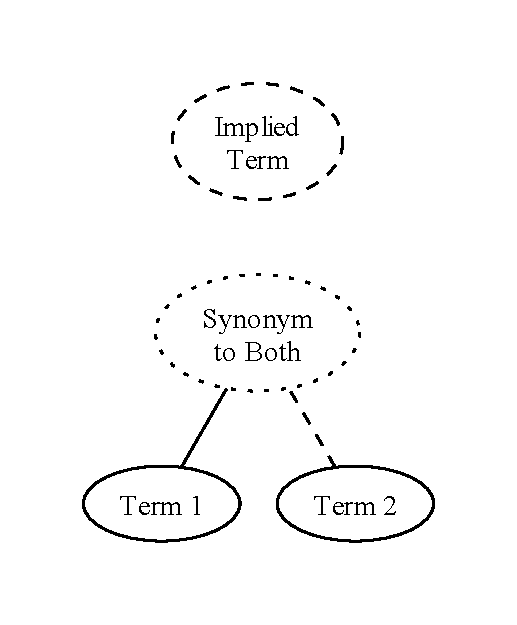
\includegraphics[width=\linewidth]{assets/graphs/manual/catRels8.pdf}
        \end{column}
        \begin{column}{.5\textwidth}
            \vspace{0.75cm}
            Dashed outlines indicate a term is \emph{implicit}.\\
            \vspace{1.3cm}
            Dotted outlines indicate a term is a \emph{synonym} to more than one term.
        \end{column}
    \end{columns}
\end{frame}

\begin{frame}{Graph of Test Approaches}
    \pause \large \centering \texttt{! Dimension too large.}
    % \includegraphics[width=0.75\textwidth]{assets/graphs/approachGraph.pdf}
\end{frame}

\begin{frame}{Graph of Test Levels}
    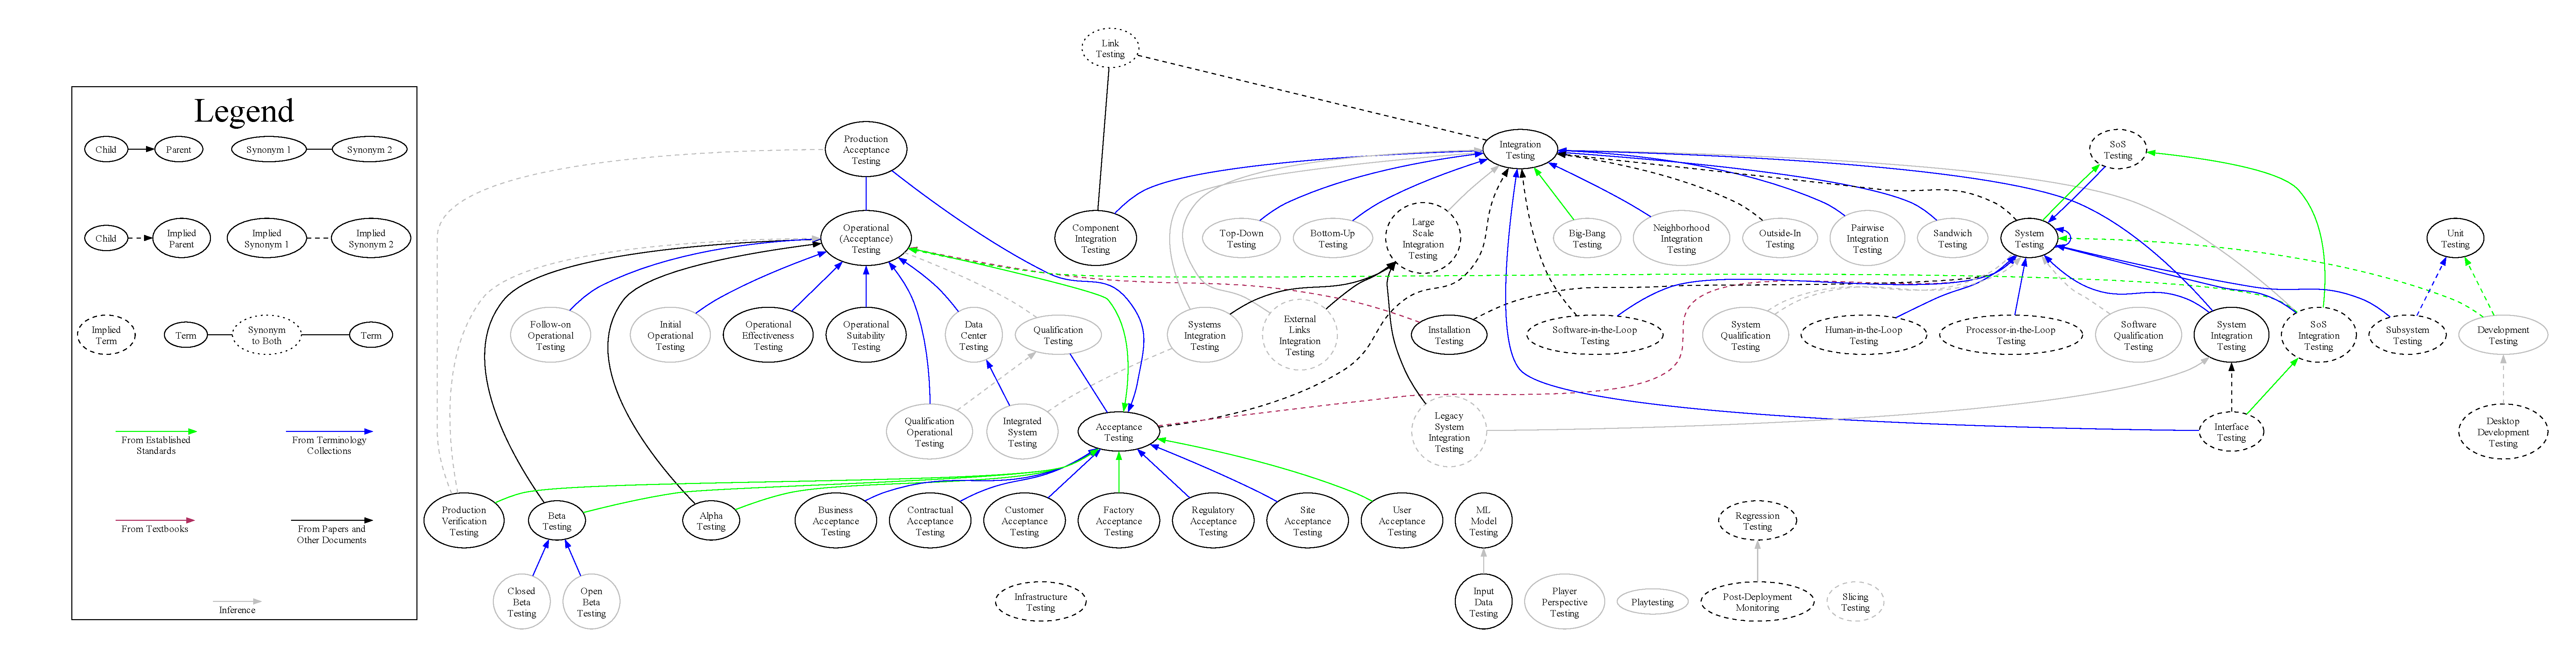
\includegraphics[width=\textwidth]{assets/graphs/levelGraph.pdf}
\end{frame}

\begin{frame}{Graph of Test Practices}
    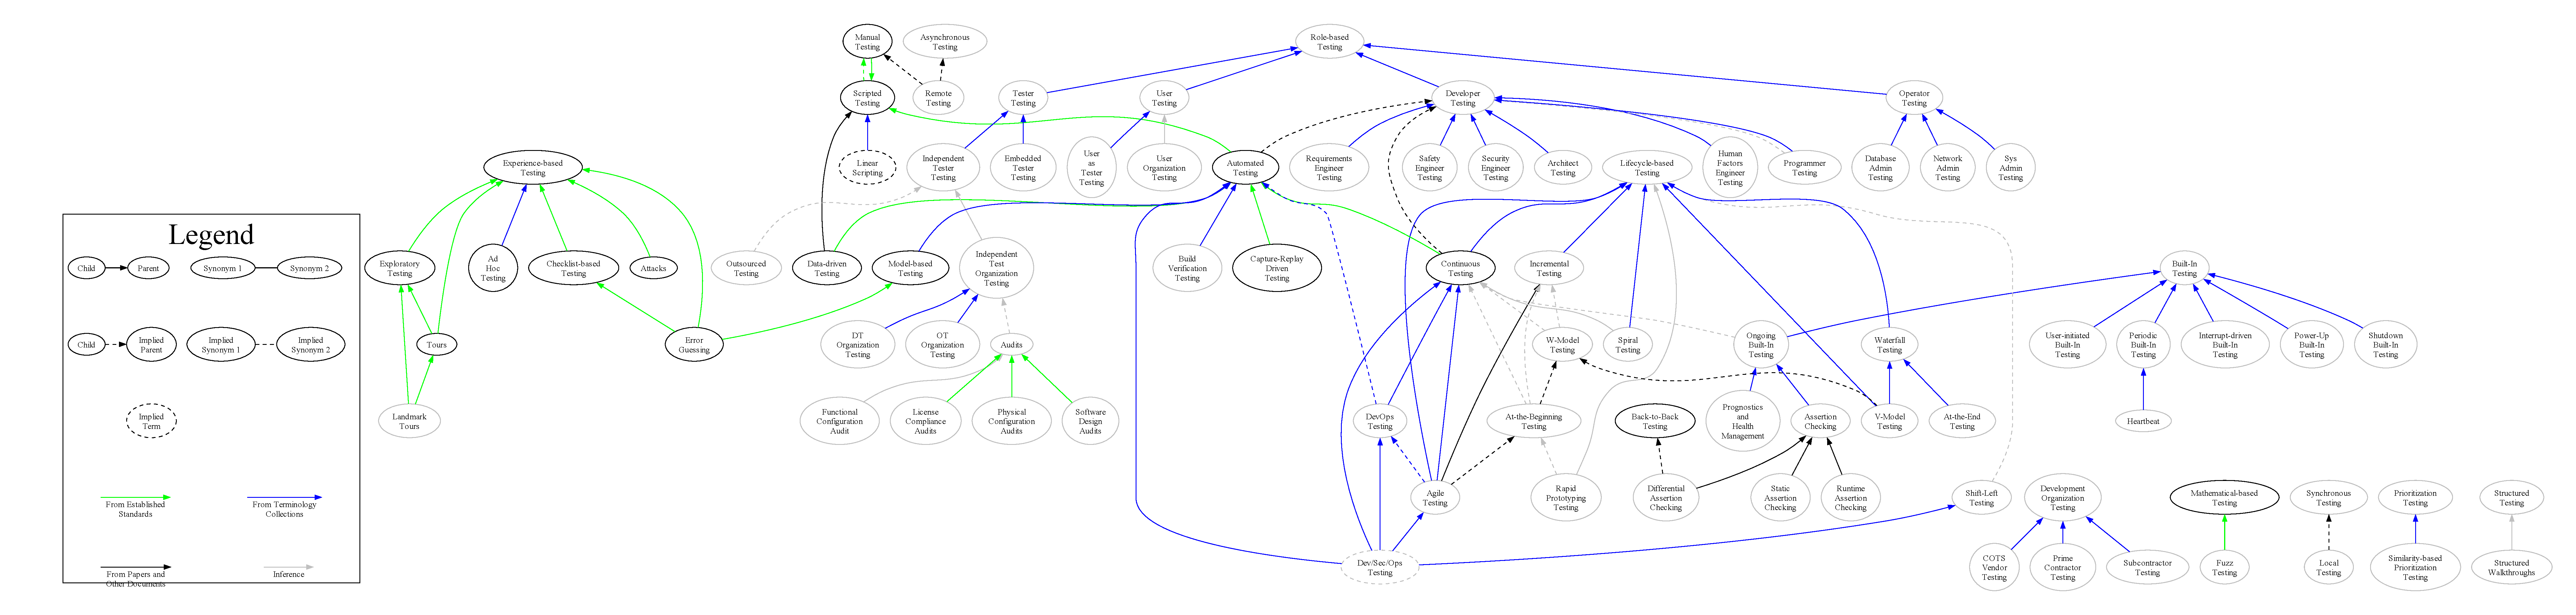
\includegraphics[width=\textwidth]{assets/graphs/practiceGraph.pdf}
\end{frame}

\begin{frame}{Graph of Test Techniques}
    \includegraphics[width=\textwidth]{assets/graphs/techniqueGraph.pdf}
\end{frame}

\begin{frame}{Graph of Test Types}
    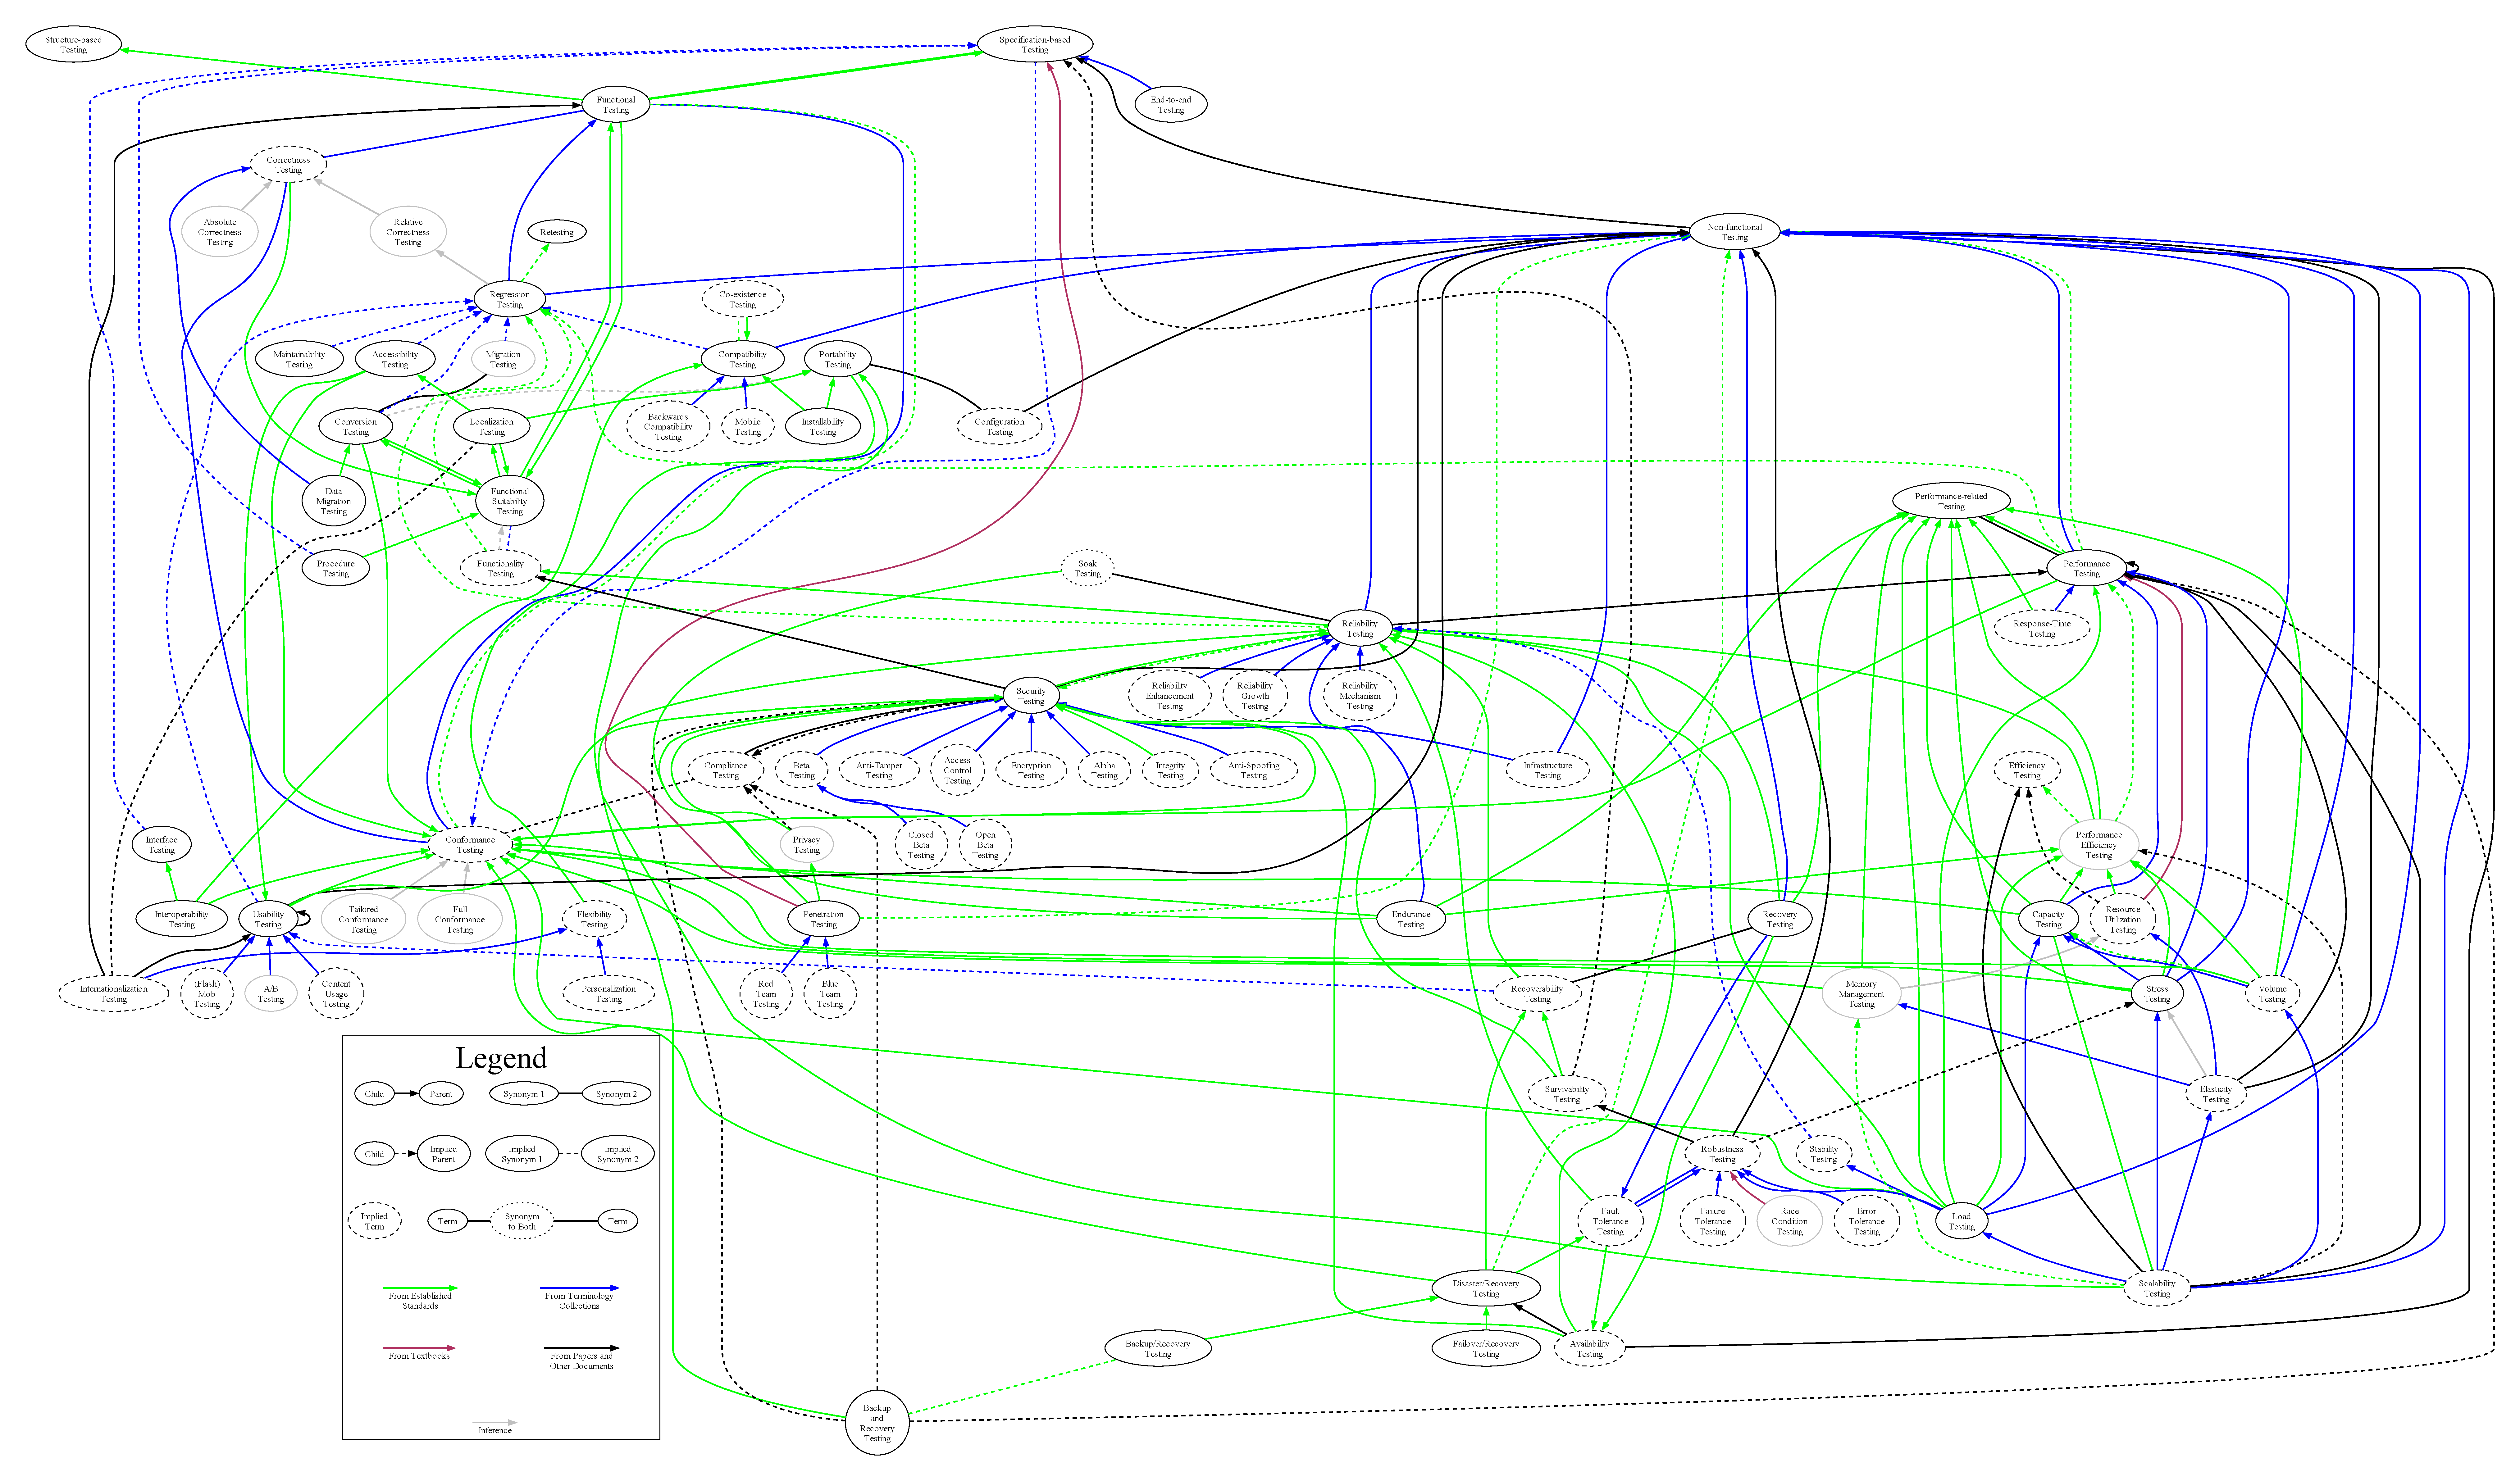
\includegraphics[width=\textwidth]{assets/graphs/typeGraph.pdf}
\end{frame}

% \begin{frame}[t]{Methodology}
%     \framesubtitle{Static Testing}
%     \begin{figure}
%         \centering
%         \includegraphics[height=0.65\textheight]{assets/images/test approach choices}
%         \caption{\tiny \citep[Fig.~2]{IEEE2022}}
%     \end{figure}
% \end{frame}

% \begin{frame}{Methodology}
%     \framesubtitle{Static Testing}
%     \begin{columns}[c]
%         \begin{column}{.3\textwidth}
%             \begin{figure}
%                 \centering
%                 \includegraphics[width=\linewidth]{assets/images/test approach static testing}
%                 \caption{\tiny Adapted from \citep[Fig.~2]{IEEE2022}}
%             \end{figure}
%         \end{column}
%         \begin{column}{.7\textwidth}
%             \begin{itemize}
%                 \item \citeauthor{IEEE2022} seem to describe ``static testing''
%                       as a separate category
%                 \item \pause Is ``static testing'' part of software testing?
%                       \vspace{-0.25cm}\begin{columns}[t]
%                           \begin{column}{.55\textwidth}
%                               \begin{center}
%                                   \textbf{Yes}
%                               \end{center} \tiny
%                               \hspace{0.75cm}\citep[pp.~16\==17]{IEEE2022} \\
%                               \hspace{0.75cm}\citep[p.~43]{IEEE2021b} \\
%                               \hspace{0.75cm}\citep[p.~5\=/2]{SWEBOK2025} \\
%                               \hspace{0.75cm}\citep[pp.~8\==9]{Gerrard2000a}
%                           \end{column}
%                           \begin{column}{.45\textwidth}
%                               \begin{center}
%                                   \hspace{-0.25cm}\textbf{No}
%                               \end{center} \tiny
%                               \citep[p.~427]{IEEE2017} \\
%                               \citep[pp.~5\=/1]{SWEBOK2025} \\
%                               \citep[p.~13]{Firesmith2015} \\
%                               \citep[p.~439]{PetersAndPedrycz2000} \\
%                               \citep[p.~222]{AmmannAndOffutt2017}
%                           \end{column}
%                       \end{columns}\vspace{0.25cm}
%                 \item \pause We record static test approaches for completeness
%                       % \item \pause Quite distinct but not necessarily orthogonal
%                       % \item \pause When considering static testing in isolation,
%                       %       related \emph{dynamic approaches} have grey backgrounds

%                       %       \vspace{-0.5cm}
%                       %       \includegraphics[width=\linewidth]{assets/graphs/manual/catRels9.pdf}
%             \end{itemize}
%         \end{column}
%     \end{columns}
% \end{frame}

% \begin{frame}{Graph of \emph{Static} Test Approaches}
%     
\includegraphics[width=\textwidth]{assets/graphs/staticGraph.pdf}
% \end{frame}

\section{Results}
\begin{frame}{Overview}
    % \onslide<1->\rqa{} \vspace*{\fill}
    % \onslide<1>\rqb{} \vspace*{\fill}
    % \onslide<1>\rqc{} \vspace*{\fill}
    % \onslide<2>
    % \vspace{-4cm}
    \begin{columns}
        \begin{column}{0.45\textwidth}
            \vspace{-1cm}
            \begin{itemize}
                \item \approachCount{} test approaches $\rightarrow$
                \item<2-> \qualityCount{} software qualities \\ \small (may imply test approaches)
                \item<3-> \flawCount{} flaws in the software testing literature
            \end{itemize}
        \end{column}
        \begin{column}{0.55\textwidth}
            \centering
            \begin{tikzpicture}
                \pie[sum=100, text=legend, thick, scale=0.5,
                every label/.style={align=left, scale=0.7}]
                {{\the\numexpr 100 - 100 * \UndefAfter/\TotalAfter}/Defined,
                {\the\numexpr 100 * \UndefAfter/\TotalAfter}/{Not defined}}
            \end{tikzpicture}
        \end{column}
    \end{columns}
\end{frame}

\begin{frame}{Flaw Summary by Source Tier}
    \begin{center}
        \begin{tikzpicture}
\begin{axis}[
width=0.8\textwidth, height=7.5cm,
yticklabels={\parbox{0.24\textwidth}{\raggedleft\papers{}},\parbox{0.24\textwidth}{\raggedleft\texts{}},\parbox{0.24\textwidth}{\raggedleft\metas{}},\parbox{0.24\textwidth}{\raggedleft\stds{}}},
ytick=data,
xlabel=\parbox{0.5\textwidth}{\centering Number of Flaws per Source Tier \\ \quad{}}, xbar, xmin=0,
nodes near coords,
every node near coord/.append style={font=\tiny},
]

\addplot[fill=blue!60] coordinates {(\the\numexpr\paperFlawMnfstBrkdwn{13},0) (\the\numexpr\textFlawMnfstBrkdwn{13},1) (\the\numexpr\metaFlawMnfstBrkdwn{13},2) (\the\numexpr\stdFlawMnfstBrkdwn{13},3)};
\end{axis}
\end{tikzpicture}


    \end{center}
\end{frame}

\begin{frame}{Normalized Flaw Summary}
    \begin{center}
        \begin{figure}[bt!]
\centering
\begin{tikzpicture}
\begin{axis}[
width=0.8\textwidth, height=7.5cm,
yticklabels={\parbox{0.24\textwidth}{\raggedleft\papers{}},\parbox{0.24\textwidth}{\raggedleft\texts{}},\parbox{0.24\textwidth}{\raggedleft\metas{}},\parbox{0.24\textwidth}{\raggedleft\stds{}}},
ytick=data,
xlabel=\parbox{0.5\textwidth}{\centering Average Number of Flaws per Document by Source Tier}, xbar, xmin=0,
nodes near coords,
every node near coord/.append style={font=\tiny,/pgf/number format/fixed,/pgf/number format/fixed zerofill,/pgf/number format/precision=1},
]
\pgfmathsetmacro{\stdResult}{\stdFlawMnfstBrkdwn{13} / \stdSources{3}}
\pgfmathsetmacro{\metaResult}{\metaFlawMnfstBrkdwn{13} / \metaSources{3}}
\pgfmathsetmacro{\textResult}{\textFlawMnfstBrkdwn{13} / \textSources{3}}
\pgfmathsetmacro{\paperResult}{\paperFlawMnfstBrkdwn{13} / \paperSources{3}}
\addplot[fill=blue!60] coordinates {(\paperResult,0) (\textResult,1) (\metaResult,2) (\stdResult,3)};
\end{axis}
\end{tikzpicture}

\end{figure}

    \end{center}
\end{frame}

\begin{frame}{Flaw Summary by Manifestation}
    \begin{center}
        \begin{figure}[bt!]
\centering
\begin{tikzpicture}
\begin{axis}[
width=0.8\textwidth, height=7.5cm,
symbolic y coords={Redundancies,Overlaps,Ambiguities,Contradictions,Omissions,Mistakes},
ytick=data,
xlabel=Flaws, xbar,
nodes near coords,
every node near coord/.append style={font=\tiny},
]
\addplot[fill=blue!60] coordinates {(7,Redundancies) (16,Overlaps) (32,Ambiguities) (175,Contradictions) (10,Omissions) (47,Mistakes)};
\end{axis}
\end{tikzpicture}
\end{figure}

    \end{center}
\end{frame}

\begin{frame}{Flaw Summary by Domain}
    \begin{center}
        \begin{figure}[bt!]
\centering
\begin{tikzpicture}
\begin{axis}[
width=0.8\textwidth, height=7.5cm,
symbolic y coords={Traceability,Scope,Labels,Definitions,Parents,Synonyms,Categories},
ytick=data,
xlabel=Flaws, xbar,
nodes near coords,
every node near coord/.append style={font=\tiny},
]
\addplot[fill=blue!60] coordinates {(7,Traceability) (5,Scope) (31,Labels) (69,Definitions) (57,Parents) (59,Synonyms) (65,Categories)};
\end{axis}
\end{tikzpicture}
\end{figure}

    \end{center}
\end{frame}

\begin{frame}{Automated Flaws}
    \begin{itemize}
        \item The literature gives some terms as a synonym to two (or more)
              disjoint, unrelated terms, making their synonym relations ambiguous
        \item \pause We include these in our generated visualizations
    \end{itemize}
    \vspace{-0.5cm}
    \begin{columns}[c]
        \begin{column}{.475\linewidth}
            \small
            \begin{table}[hbtp!]
                \centering
                \begin{tabularx}{\textwidth}{c>{\raggedleft\arraybackslash}X} \hline
                    Name & Synonym(s)                                   \\ \hline
                    E    & F (Author, 2022; implied by StdAuthor, 2021) \\
                    G    & F (Author, 2017), H (implied by 2022)        \\
                    H    & X (StdAuthor, 2021)                          \\ \hline
                \end{tabularx}
            \end{table}
        \end{column}
        \begin{column}{.5\linewidth}
            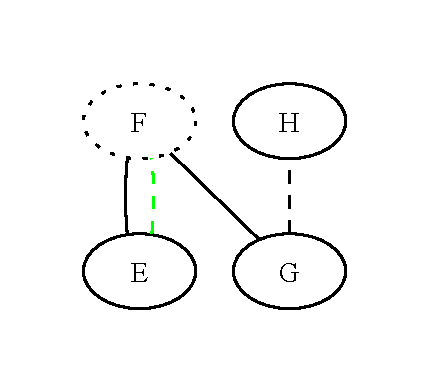
\includegraphics[width=\textwidth]{assets/graphs/SynExampleGlossaryGraph.pdf}
        \end{column}
    \end{columns} %\pause
    \vspace{-0.25cm}
\end{frame}

\begin{frame}{Automated Flaws}
    Prominent examples of these ``multi-synonyms'': \vspace{0.25cm}
    \begin{enumerate}
        % \item \textbf{Invalid Testing:} \hfill \textbf{Source(s)}
        %       \begin{itemize}
        %           \item Error Tolerance Testing {\hfill \tiny \citep[p.~45]{Kam2008}}
        %           \item Negative Testing {\hfill \tiny \citepISTQB{}}
        %       \end{itemize} \pause
        \item \textbf{Soak Testing:} \hfill \textbf{Source(s)}
              \begin{itemize}
                  \item Endurance Testing {\hfill \tiny \citep[p.~39]{IEEE2021c}}
                  \item Reliability Testing {\hfill \tiny (\citealp[Tab.~2]{Gerrard2000a};
                                \citeyear[Tab.~1, p.~26]{Gerrard2000b})}
              \end{itemize} \pause
        \item \textbf{Functional Testing:}
              \begin{itemize}
                  \item Behavioural Testing {\hfill \tiny \citep[p.~45]{Kam2008}}
                  \item Correctness Testing {\hfill \tiny \citep[p.~5\=/7]{SWEBOK2024}}
                  \item Specification-based Testing {\hfill \tiny (\citealp[p.~196]{IEEE2017}; \dots{})}
                        % \citealp[pp.~44\==45]{Kam2008}; \citealp[p.~399]{vanVliet2000})}
                        % implied by \citealp[p.~129]{IEEE2021c}; \citeyear[p.~431]{IEEE2017})}
              \end{itemize} \pause
        \item \textbf{Link Testing:}
              \begin{itemize}
                  \item Branch Testing {\hfill \tiny (implied by \citealp[p.~24]{IEEE2021c})}
                  \item Component Integration Testing {\hfill \tiny \citep[p.~45]{Kam2008}}
                  \item Integration Testing {\hfill \tiny (implied by \citealp[p.~13]{Gerrard2000a})}
              \end{itemize}
    \end{enumerate}
\end{frame}


%   \begin{figure}
%       %   \vspace{-1mm}
%       \includegraphics[width=.8\textwidth]{assets/stable.png}
%       %   \vspace{-3mm}
%       \caption{Contents of \texttt{stable}}
%       \vspace{-1mm}
%   \end{figure}

%   \lstinputlisting[
%       title=An example log,
%       captionpos=b,
%       language={},
%       basicstyle=\tiny, % TODO: reduce font size?
%       breakatwhitespace=true,
%       showstringspaces=false
%   ]{assets/log.txt}

% \onslide<7-|handout:1>\begin{block}{}
%     {"The information you have should be just as useful for generating
%         tests as it should be for manually running them."}
%     \vspace{3mm}
%     \hspace\fill{\small--- Dr.~Jacques Carette}
% \end{block}


%%%%%%%%%%%%%%%%%%%%%%%%%%%%%%%%%%%%%%%%%%%%%%%%%%%%%%%%%%%%%%%%%%%%%%%%%%%%%%%
%% ACKNOWLEDGEMENTS
%%%%%%%%%%%%%%%%%%%%%%%%%%%%%%%%%%%%%%%%%%%%%%%%%%%%%%%%%%%%%%%%%%%%%%%%%%%%%%%

\begin{frame}
    \frametitle{Acknowledgment}

    \begin{itemize}
        \item \supersAck{}
              \begin{itemize}
                  \item They have helped me refine the scope of this project
                  \item Dr.~Smith first suggested generating test cases back in 2020!
              \end{itemize}
        \item<2-> The format of this presentation was \emph{heavily} based on
              a previous presentation by Jason Balaci, who also provided a
              great thesis template
        \item<3-> The past and current Drasil team have created a truly amazing
              framework!
    \end{itemize}
\end{frame}

%%%%%%%%%%%%%%%%%%%%%%%%%%%%%%%%%%%%%%%%%%%%%%%%%%%%%%%%%%%%%%%%%%%%%%%%%%%%%%%
%% A FINAL THANK YOU
%%%%%%%%%%%%%%%%%%%%%%%%%%%%%%%%%%%%%%%%%%%%%%%%%%%%%%%%%%%%%%%%%%%%%%%%%%%%%%%

\begin{frame}
    \center
    \huge{Thank you!}\\
    \normalsize{Questions?}
\end{frame}

%%%%%%%%%%%%%%%%%%%%%%%%%%%%%%%%%%%%%%%%%%%%%%%%%%%%%%%%%%%%%%%%%%%%%%%%%%%%%%%
%% REFERENCES
%%%%%%%%%%%%%%%%%%%%%%%%%%%%%%%%%%%%%%%%%%%%%%%%%%%%%%%%%%%%%%%%%%%%%%%%%%%%%%%

% From https://tex.stackexchange.com/a/457255/192195
\setbeamertemplate{page number in head/foot}{}

\begin{frame}[allowframebreaks,noframenumbering]
    \frametitle{References}

    \bibliography{references,seminar_images}
\end{frame}

\end{document}
